\chapter{PictUp! Arquitectura e implementación}
\label{cap:arquitectura}


%\begin{resumen} 
%La arquitectura de la aplicación (Sección \ref{cap5:arquitectura}), funcionamiento de la cuadrícula (Sección \ref{cap5:cuadricula} ), el desarrollo de las funcionalidades implementadas (Secciones de \ref{cap5:buscador} a \ref{cap5:descargar}), las funcionalidades no implementadas (Sección \ref{cap5:noimplementadas} ) y el despliegue (Sección \ref{cap5:despliegue}). Por último se explicará cómo se ha organizado el desarrollo y control de versiones de PictUp! (Sección \ref{cap5:controlversiones} ) 

%\end{resumen}

\section{Introducción}

Una vez especificados las características y requisitos a implementar, se pudo empezar a desarrollar la arquitectura de la aplicación y la implementación de dichas características. Desde un primer momento, se determinó que la aplicación tendrá una barra de herramientas donde se incluirán distintas funcionalidades como buscar pictogramas o realizar traducción de frases. También se incluirá una cuadrícula donde se podrán poner sobre ella los distintos elementos de los materiales pictográficos. El conjunto de estas funcionalidades permitirá crear tableros pictográficos. A continuación se explicará la jerarquía utilizada en la aplicación, las funcionalidades y los ítems disponibles. 

\section{Arquitectura}
\label{cap5:arquitectura}

La arquitectura de PictUp! puede distinguirse a dos niveles. A nivel interno se especificará la arquitectura de un componente de React, pues todos ellos cuentan con un diseño similar. A nivel externo, se especificará cómo las distintas componentes desarrolladas interactúan entre ellas y se verá un esquema de la jerarquía de éstas. 


\subsection{Arquitectura interna}

La aplicación está compuesta principalmente por componentes\footnote{\url{https://reactjs.org/docs/react-component.html\#gatsby-focus-wrapper}} de React, los cuales son clases que deben contar obligatoriamente con un método \texttt{render()} y de manera opcional puede contar con el objeto \texttt{state}\footnote{\url{https://reactjs.org/docs/faq-state.html\#what-does-setstate-do}}. El objeto \texttt{state} permite almacenar distintas variables. La principal característica de este objeto es que al actualizar el valor de cualquiera de sus variables definidas en su interior, el componente vuelve a renderizarse. Para actualizar el valor de cualquier variable del \texttt{state}, ha de realizarse mediante el método \texttt{setState()}. Este método se realiza de manera asíncrona, por lo que los valores de \texttt{state} generalmente van ligados a datos que serán mostrados en el método renderización. De esta manera,  \texttt{state} será de gran ayuda para actualizar la interfaz con la que interactúa el usuario. 
Los componentes pueden tener variables fuera del objeto \texttt{state} si no se va a utilizar para la renderización.  


El método \texttt{render()}\footnote{\url{https://es.reactjs.org/docs/rendering-elements.html }} se encarga de renderizar el html del componente. Dentro del render se podrán incluir los atributos que se hayan definido en el \texttt{state} u otros elementos como botones, selectores o campos de texto. 
La característica principal que ofrece este método de React es que si se modifica un atributo del \texttt{state} del componente, automáticamente se mostrará en el navegador en nuevo valor que haya tomado. Otra característica que ofrece React es poder llamar desde el render a funciones externas dentro del componente que se encargan de devolver el fragmento html deseado. Esto sirve para organizar mejor el contenido y crear render condicionales, es decir, mostrar un contenido u otro en función de los valores que tomen un atributo del \texttt{state}.
Además también se puede incluir dentro de la función render otros componentes de React, que pasará a ser el componente hija que puede recibir parámetros de entrada o salida mediante \texttt{props}. Las \texttt{props} son atributos de React que permiten enviar información entre componentes padres e hijos. Para acceder a los parámetros enviados desde el componente padre se hará utilizando \texttt{this.props}\footnote{\url{https://es.reactjs.org/docs/components-and-props.html }}.

\subsection{Arquitectura externa}

Una vez vista la estructura de un componente, se puede ver en la Figura \ref{fig:pantallaprincipal} la pantalla principal de PictUp!, la cual está compuesta por multitud de componentes. Estos son agrupados y gestionados mediante el componente Main. Como se puede ver, se pueden distinguir varios apartados bien diferenciados en pantalla principal: 

% TODO: \usepackage{graphicx} required
\begin{figure}[h!]
	\centering
	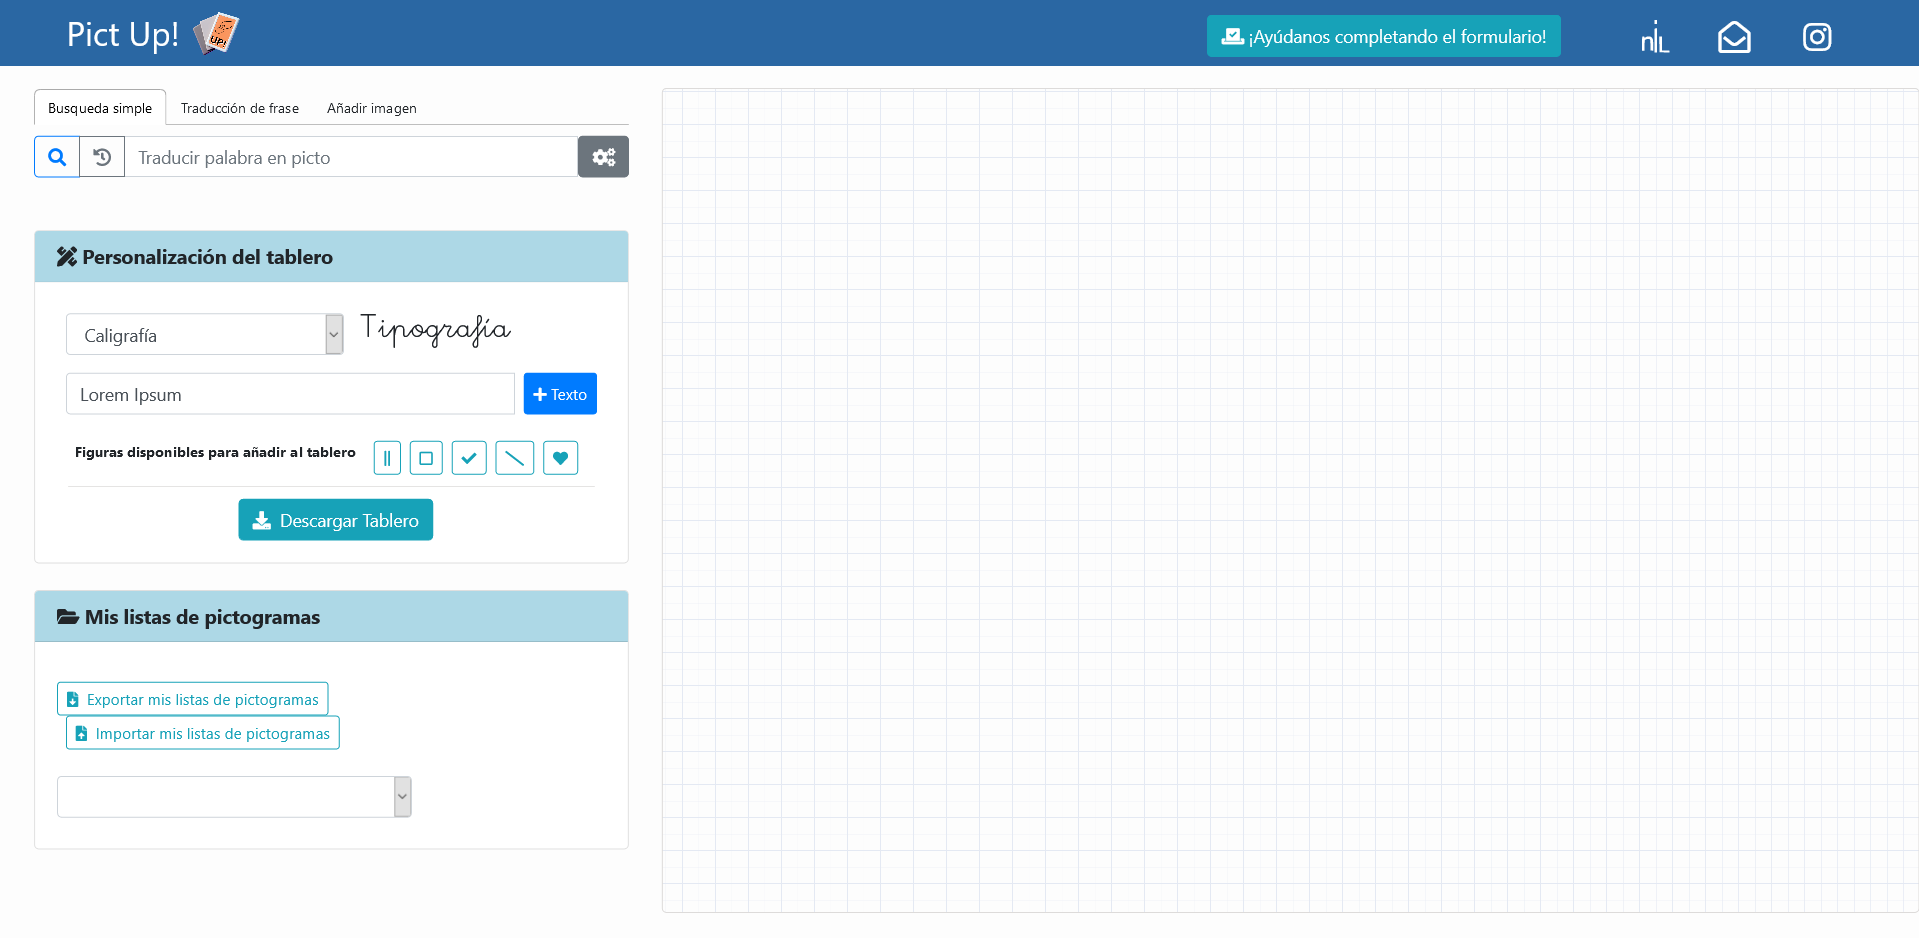
\includegraphics[width=\linewidth]{Imagenes/Bitmap/pantallaprincipal}
	\caption{Vista inicial de PictUp!.}
	\label{fig:pantallaprincipal}
\end{figure}

\begin{itemize}
	\item \textbf{Navbar}: se encuentra en la zona superior y en ella vemos el nombre de la aplicación junto con su imagen. También se incluye información de contacto.
	
	
	\item \textbf{Barra de Herramientas}: en la zona izquierda de la aplicación se agrupan todas las herramientas disponibles. 
	Estas son componentes que ofrecen una interfaz al usuario para añadir elementos a la cuadrícula. Algunas de estas herramientas cuentan con pantallas auxiliares en forma de modal, como es el caso de búsqueda de pictogramas o la función de descargar tablero. Cada una de las herramientas pueden retornar elementos con representación en la cuadrícula, los cuales serán denominados ítems. La información asociada a cada uno de estos ítems serán almacenados en el \texttt{state} de Main dependiendo de su tipo.
	
	\item \textbf{Tablero}: es el componente que mayor espacio abarca de la página, siendo la zona donde se desplazarán los elementos generados por las herramientas. El tablero se muestra en forma de cuadrícula. Sobre ésta se colocarán los ítems que tenga almacenados Main en su \texttt{state}.  Como se puede ver en la Figura \ref{fig:items} existen distintos tipos de ítem, como pictograma, texto o icono. Cada ítem está adecuado en función del tipo de contenido que se vaya a mostrar. Asimismo, los ítems cuentan con funcionalidades que les permiten cambiar sus propiedades. Por ejemplo, el que representa texto podrá modificar el tamaño de letra y contenido.  
	
\end{itemize}


	

% TODO: \usepackage{graphicx} required
\begin{figure}[h!]
	\centering
	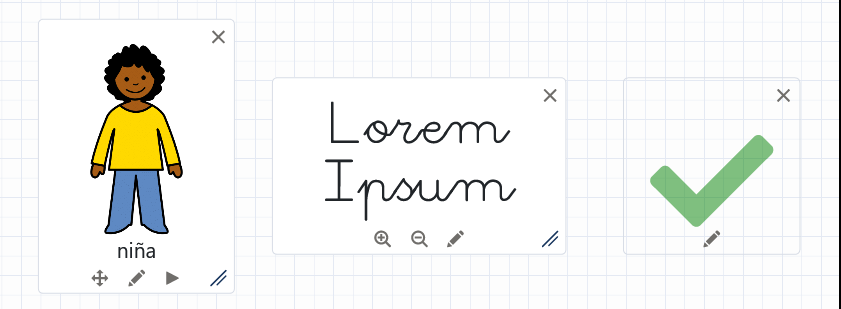
\includegraphics[width=0.7\linewidth]{Imagenes/Bitmap/items}
	\caption{Ejemplos de Ítems.}
	\label{fig:items}
\end{figure}
	

Para esquematizar cómo interactúan la distintas componentes, la Figura \ref{fig:diagramaarquitectura} se representan las distintas componentes de la aplicación y cómo se relacionan entre sí.

% TODO: \usepackage{graphicx} required
\begin{figure}[h!]
	\centering
	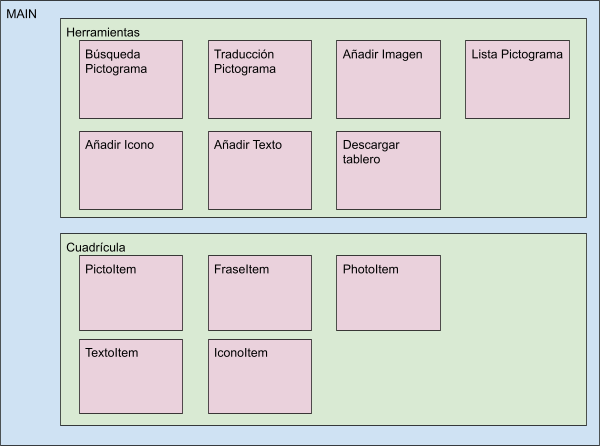
\includegraphics[width=\linewidth]{Imagenes/Bitmap/diagramaarquitectura}
	\caption{Diagrama de los componentes de la aplicación.}
	\label{fig:diagramaarquitectura}
\end{figure}


\subsection{Cuadrícula}
\label{cap5:cuadricula}

En esta sección se explicará el funcionamiento en detalle de la cuadrícula. Para facilitar la tarea de desplazar elementos en un espacio, el proyecto de la cuadrícula fue clonado del proyecto  \textit{dnd-a11y-patterns}\footnote{\url{https://github.com/salesforce-ux/dnd-a11y-patterns}} que contaba con componentes que permitían desplazarse de distintas maneras. Cuenta con una licencia \textit{BSD 3-Clause} que permite libertad de modificación y distribución.


El empezar desde este proyecto facilitó el  tratamiento de eventos de desplazamiento (Drag and Drop), los cuales iban a ser de gran importancia para mover los distintos ítems de la aplicación. Además de gestionar estos eventos, cuenta con muchos parámetros que han sido modificados, como el ancho y alto inicial de cada ítem o la posibilidad de mantener la proporción de un ítem al ser redimensionado.

El componente de cuadrícula o canvas es una cuadrícula de la cual se puede modificar su tamaño mediante la cantidad de filas y columnas y el intervalo en píxeles entre estas. El tamaño de la cuadrícula fue ajustado para que abarque el mayor ancho y alto posible teniendo en cuenta el espacio reservado para la barra de herramientas. Sobre esta componente canvas se colocarán otros componentes, que serán los ítems. 

Los ítems son elementos que se pueden colocar sobre la cuadrícula de la aplicación y permiten ser desplazados y redimensionados. Al haber distintos tipos de ítems cada uno de ellos mostrará el contenido de distintas maneras. Por ejemplo, los PictoItem tendrán en su interior una imagen del pictograma mientras que el TextoItem simplemente tendrá un texto. Dado que los ítems se encuentran dentro de la clase cuadrícula, reciben atributos tales como el intervalo de la cuadrícula. Esto permitirá a los ítems desplazarse en función de dicho intervalo, ayudando al usuario a mover y redimensionar los ítems con mayor precisión. Al existir distintos elementos que se pueden colocar en la cuadrícula (pictos, fotos, figuras, texto, etc), cada uno cuenta con su propio  ítem que los representa (PictoItem, FotoItem, FigureItem, etc).


Cada ítem cuenta con un renderizado y funcionalidades adecuadas para cada elemento. La mayoría de estos ítems tienen en común los botones visibles en la Figura \ref{fig:botonesitem}, como desplazar y redimensionar (los cuales habilitan la utilización de las teclas del teclado para realizar estas dos acciones con una mayor precisión), y otro botón en la esquina superior derecha para eliminar el pictograma de la cuadrícula. Cuando se pulsa, se envía al componente padre el item seleccionado para ser eliminado de la lista donde se encuentre.

% TODO: \usepackage{graphicx} required
\begin{figure}[h!]
	\centering
	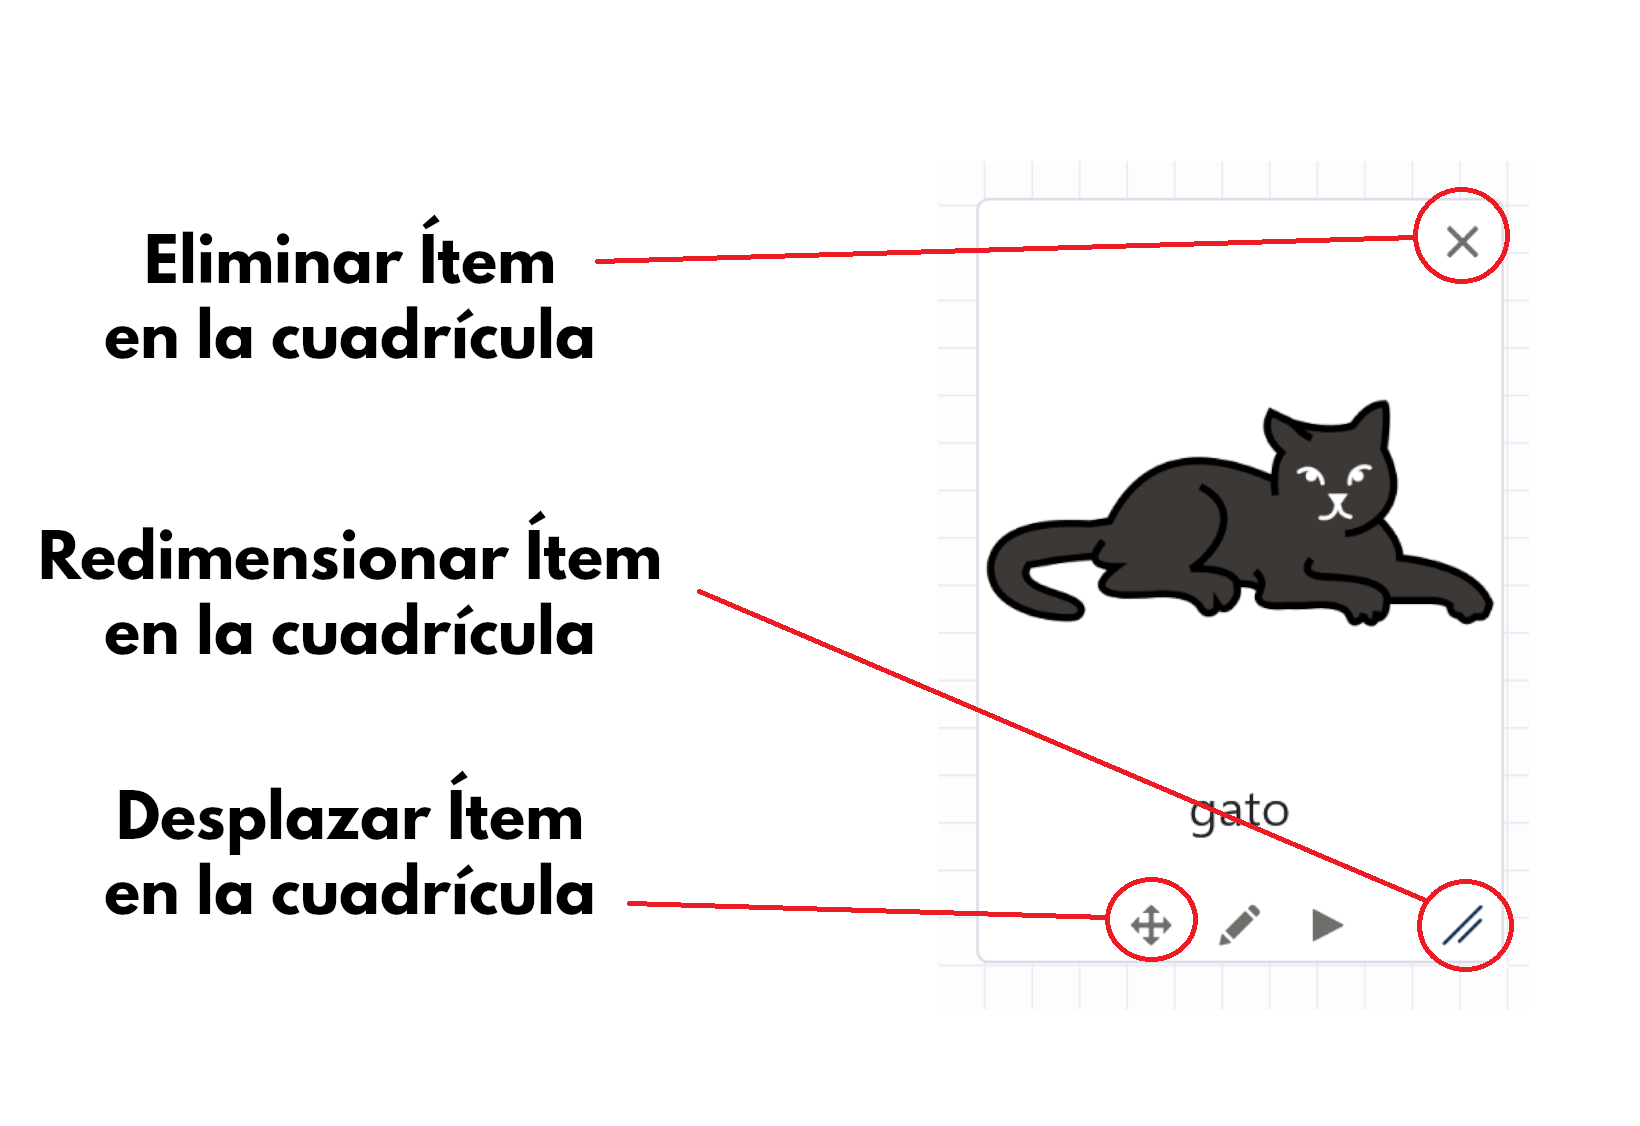
\includegraphics[width=0.7\linewidth]{Imagenes/Bitmap/botonesItem}
	\caption{Ejemplo de botones de redimensión y desplazamiento.}
	\label{fig:botonesitem}
\end{figure}


Una vez explicado cómo funciona a nivel interno la aplicación, se procederá a explicar el funcionamiento de las distintas herramientas y las posibilidades que ofrecen. En caso de que una herramienta cree un ítem en la cuadrícula, se explicarán sus opciones y posibilidades. Asimismo se especificarán las reglas de diseño utilizadas en cada una de ellas (ver Sección \ref{cap5:reglasBusqueda}).



%\section*{Funcionalidades de PictUp!}

%A continuación se explicarán las funcionalidades que podemos encontrar en la aplicación, su representación en caso de contar con un item y que reglas de diseño son utilizadas.

\section{Buscador de pictogramas}
\label{cap5:buscador}
El buscador de pictogramas es la herramienta que muestra los distintos pictogramas que se asocian a una palabra mediante la API de \textit{ARASAAC}. Como se puede ver en la Figura \ref{fig:buscarpicto2}, el componente, aparte de contar con el buscador identificado mediante el icono de la lupa, también tiene un historial que almacena los pictogramas recientemente añadidos asociado al icono del reloj. Además, a la derecha del buscador se encuentra la opción de preajuste de pictogramas identificado con el icono de los engranajes. Estas dos opciones son muy convenientes de cara a añadir un pictograma al tablero. 


% TODO: \usepackage{graphicx} required
\begin{figure}[h!]
	\centering
	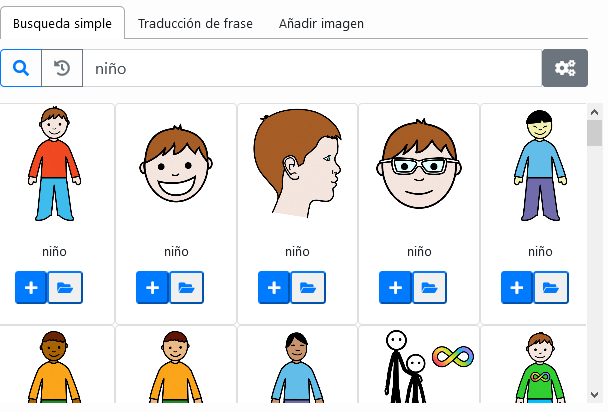
\includegraphics[width=0.7\linewidth]{Imagenes/Bitmap/buscarPicto2}
	\caption{Vista del componente de búsqueda de pictogramas.}
	\label{fig:buscarpicto2}
\end{figure}


Para empezar se va a explicar cómo está estructurado el componente de búsqueda de pictogramas. En la variable \texttt{state} del componente se almacenará:

\begin{itemize}
	\item La palabra de la que se quiere obtener sus pictogramas.
	\item Los pictogramas encontrados por la consulta.
	\item El preajuste de los pictos, donde se especifica cómo se van a mostrar los pictogramas.
	\item Flags de control, para indicar si se ha completado la búsqueda, está abierto el modal, o si se ha seleccionado el historial.     
\end{itemize}

Respecto a las funciones que abarca el componente, se pueden distinguir tres tipos: las que realizan las peticiones a la API de ARASAAC, las que gestionan los resultados de las peticiones y dos métodos de renderización. El primer método se encargará de mostrar la barra de búsqueda, que cuenta con los botones mencionados anteriormente (buscar, historial, preajuste de pictogramas) que llamarán a sus funciones asociadas. El segundo método de renderización recibe como parámetro de entrada una lista de pictogramas y los mostrará junto a los botones para añadirlos a la cuadrícula o lista de pictogramas. A continuación se explicará el funcionamiento de estas funcionalidades. 


\subsection{Búsqueda}

Al pulsar sobre el icono de la lupa o pulsar intro se lanza la consulta a la API de ARASAAC por el método \texttt{bestSearch} mediante Fetch\footnote{\url{https://developer.mozilla.org/es/docs/Web/API/Fetch_API/Using_Fetch}}. El fetching puede realizar y recibir peticiones en JavaScript de manera asíncrona de manera sencilla. De esta manera, hasta no recibir una respuesta en forma de JSON con la lista de pictogramas, no se enviará al método de renderización de pictogramas. 

Cuando llegue dicha lista a este método, será cuando se use el preajuste para que la apariencia de los pictogramas sea de acuerdo a lo marcado por el usuario. En la Sección \ref{preajuste} se explica en detalle cómo se obtiene y modifica la URL que se muestra. Con la URL creada, se mostrarán los pictogramas devueltos por la API. El método de renderización añade a cada pictograma dos botones: añadir a la cuadrícula y guardar en una lista de pictos. En ambos casos se enviará el pictograma a el componente padre donde será tratado de maneras distintas. Respecto a cómo será tratado el pictograma al añadirlo a una lista se verá detalladamente en la Sección \ref{listapictos} (Lista de Pictos).

En caso de añadirlo a la cuadrícula, primero guardará el pictograma en el historial de pictos y posteriormente se enviará a el componente padre (dragOnCanvas).  Éste recibiría el pictograma que ha devuelto la API de ARASAAC junto a sus parámetros y el preajuste aplicado a dicho picto. Antes de ver el funcionamiento del nuevo ítem que aparecerá en la cuadrícula, es importante conocer el funcionamiento del preajuste y el historial.


\subsection{Preajuste}
\label{preajuste}

La manera de obtener la dirección URL de una imagen tiene dos maneras de abordarse. En un primer lugar se podría poner simplemente la URL “https:// api.arasaac.org/api/pictograms/” junto al identificador del pictograma. De esta manera simplemente se mostraría el pictograma pero perderíamos la valiosa posibilidad de editar un pictograma que ofrece ARASAAC.

Para poder optar a las modificaciones, se ha de modificar la URL de una manera concreta. Desde la propia API se especifican los atributos modificables que se pueden aplicar a todos los pictogramas:  


\begin{itemize}
	\item \textbf{action}: añade una flecha para indicar que una acción se da en el futuro o en el pasado.
	\item \textbf{plural}: añade un “+” en la esquina superior derecha.
	\item \textbf{nocolor}: muestra el pictograma en blanco y negro.
	
\end{itemize}

Existen otras dos modificaciones que solo son aplicables a los pictogramas cuyos parámetros “hair” y “skin” estén marcados como “true“.


\begin{itemize}
	\item \textbf{hair}: si un pictograma tiene pelo su color puede ser uno de entre seis colores posibles asociado a su valor hexadecimal: moreno, rubio, pelirrojo, etc.
	
	\item \textbf{skin}: si el pictograma contiene una persona se puede modificar el tono de piel de entre cinco posibles, especificados mediante su valor hexadecimal.
	
\end{itemize}

Es aquí donde entra en acción el preajuste de pictogramas, ofreciendo al usuario una interfaz donde modificar la apariencia de los pictogramas que se buscan y posteriormente se añaden. Al pulsar sobre el botón del engranaje, visible en la barra de búsqueda de la Figura \ref{fig:buscarpicto2}, se abre el modal que se ve en la Figura \ref{fig:modalpreajustepicto}. El modal en sí es otra componente que recibe como parámetro de entrada los preajustes ya establecidos y devuelve los nuevos preajustes. Los preajustes son los atributos vistos anteriormente: color de pelo, tono de piel, color y plural.

% TODO: \usepackage{graphicx} required
\begin{figure}[h!]
	\centering
	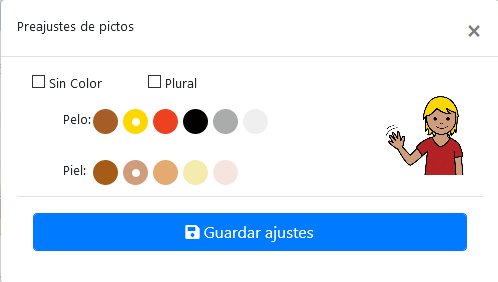
\includegraphics[width=0.7\linewidth]{Imagenes/Bitmap/modalPreajustePicto}
	\caption{Vista del modal del preajuste de pictos con las opciones color de pelo rubio y piel morena marcadas.}
	\label{fig:modalpreajustepicto}
\end{figure}



La interfaz del modal consiste en dos filas. La primera para los checkbox que marcan las opciones de plural y color, las cuales pueden estar activadas o desactivadas. La segunda fila es para elegir una de entre las distintas opciones de color disponibles tanto para el tono de piel como para el color de pelo. Está dispuesto de esa manera ya que si se marca algún checkbox, los botones radiales desaparecen. Esto se debe a que no es posible tener por ejemplo, un pictograma sin color y color de pelo rubio, previniendo así combinaciones que no estén disponibles.

A la izquierda cuenta con una previsualización para que el usuario conozca cómo afectan los atributos seleccionados al pictograma. Una vez el usuario esté conforme con los cambios, se envían al componente búsqueda de pictogramas las opciones seleccionadas.

Respecto a la construcción de las URLs se realiza de la siguiente manera:

\begin{enumerate}
	\item Se parte de la URL \texttt{https://static.arasaac.org/pictograms/id/id + \{options\} + \_500.png}. En la variable \texttt{options} se añadirán las opciones que modifiquen al pictograma.
	
	
	\item Dichas opciones deben estar  en un orden concreto utilizando los valores obtenidos del preajuste y el pictograma a crear. Por ejemplo, si se va a crear la URL del  pictograma “avión”, los ajustes relacionados con el color de pelo o piel no se aplicarían, ya que el picto no lo permite.
	 
	\item Un resultado posible para \texttt{option} sería: \\
	\texttt{\_action-future\_hair-020100\_skin-A65C17}. \\Respecto al significado de cada etiqueta: \texttt{\_action-future} añade la flecha en la esquina superior derecha indicando futuro y \texttt{hair}, y \texttt{skin} van asociados a su color hexadecimal correspondiente obtenido del preajuste. Si la etiqueta de \texttt{hair} fuera antes que la de \texttt{skin}, la URL creada no funciona. De ahí la importancia del orden.
	
	\item La URL creada se usa en cada pictograma mostrado en función de los preajustes, tal y como se puede observar en la Figura \ref{fig:buscarpictopreajuste}.
	
\end{enumerate}



% TODO: \usepackage{graphicx} required
\begin{figure}[h!]
	\centering
	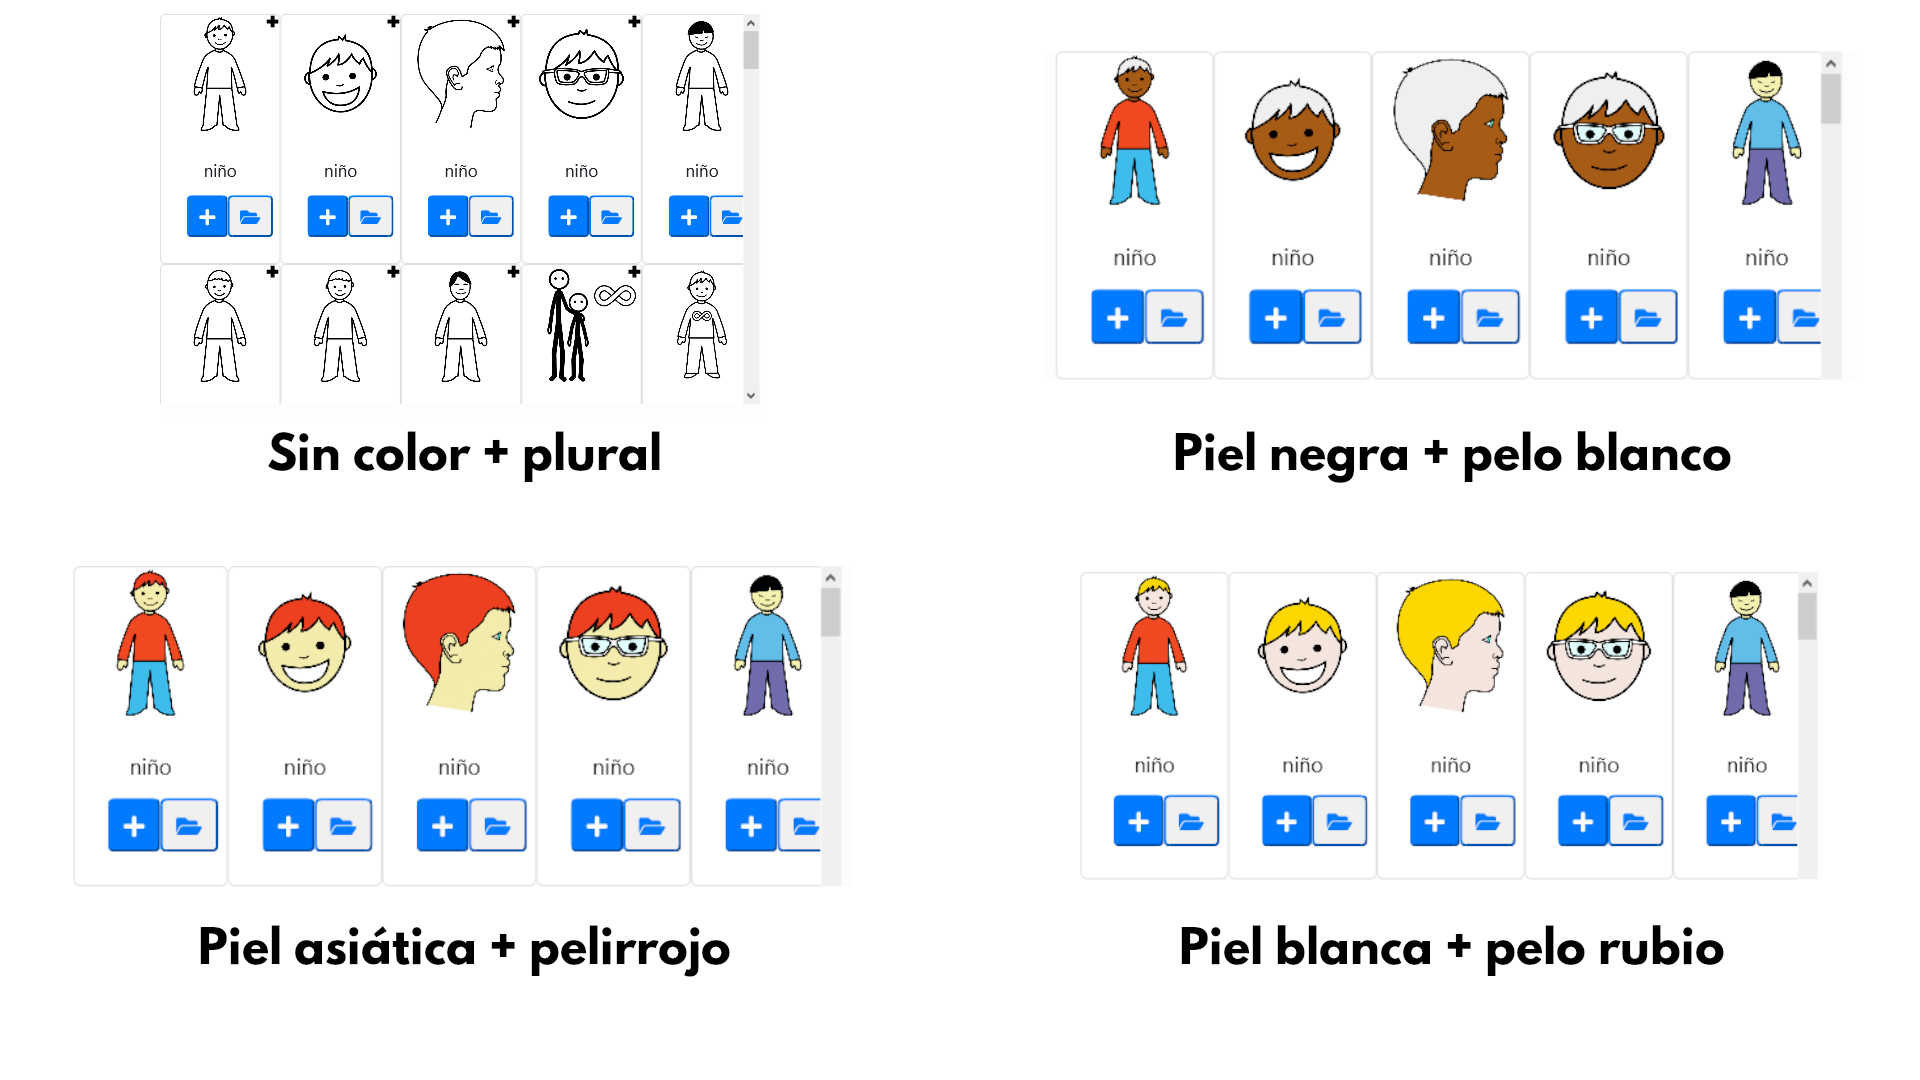
\includegraphics[width=0.9\linewidth]{Imagenes/Bitmap/buscarPictoPreajuste}
	\caption{Ejemplos de tipos de distintas combinaciones de preajuste.}
	\label{fig:buscarpictopreajuste}
\end{figure}



\subsection{Historial de pictos}

Al añadir un pictograma al tablero, dicho pictograma se guarda en el historial que se mantiene entre sesiones. Para ello se ha utilizado LocalStorage\footnote{\url{https://developer.mozilla.org/en-US/docs/Web/API/Window/localStorage}}, el cual almacena una lista en la variable “recentPictos”. Dicha lista está compuesta por el objeto devuelto por la API de ARASAAC parseado a \texttt{string}, ya que los valores almacenados en LocalStorage solo pueden estar en formato \texttt{UTF-16 DOMString} que utiliza dos bytes por carácter.

Al pulsar sobre el botón de historial se cargarán y mostrarán todos los pictogramas encontrados en \texttt{recentPictos}. En caso que el historial esté vacío, se mostrará un mensaje indicándolo. Al igual que en el caso de la búsqueda, los pictogramas del historial se podrán añadir al tablero o a una lista, y son susceptibles del preajuste de pictogramas.

Es importante destacar que al realizar las pruebas se puso un límite a los pictogramas que se pudieran guardar en el historial. A partir de 300 aparecían pérdidas de rendimiento llegando a detener momentáneamente la página, motivo por el cual se redujo a 50.

\subsection{PictoItem}

PictoItem es el componente asignado para representar un pictograma en la cuadrícula. En la Figura \ref{fig:pictoitemmodificado} se puede ver su representación en el tablero: la mayor parte del componente lo abarca el pictograma, y debajo está su nombre. Las funcionalidades que tiene este PictoItem son la de editar el picto mediante el botón del lápiz y la de reproducir el sonido de su texto asociado mediante el botón \textit{play}. Respecto a su estructura interna, en su \texttt{state} almacena el objeto picto obtenido anteriormente de la API de ARASAAC, el preajuste asignado y \textit{flags} que indican si su modal de edición de  picto es visible o no. A continuación se detallarán las funcionalidades que ofrece  PictoItem.


% TODO: \usepackage{graphicx} required
\begin{figure}[h!]
	\centering
	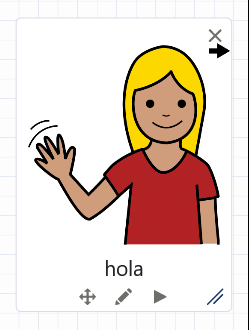
\includegraphics[width=0.4\linewidth]{Imagenes/Bitmap/pictoItemModificado}
	\caption{Vista de un PictoItem en la cuadrícula con preajuste de pelo y piel. }
	\label{fig:pictoitemmodificado}
\end{figure}





\subsubsection{Editar Picto}

Tiene un funcionamiento igual al de preajuste de picto aunque se han añadido dos opciones más. Tal y como se puede ver en la Figura \ref{fig:modaleditarpicto}, éstas son el selector de tiempo verbal y  borde. El motivo de aparición de estas dos opciones en este modal y no en el preajuste es la de no abrumar al usuario. El Borde puede ser de utilidad para los usuarios que quieran resaltar el tipo de pictograma mediante un color. El selector de tiempo verbal sirve para indicar si una acción toma lugar en presente, pasado o futuro.

% TODO: \usepackage{graphicx} required
\begin{figure}[h!]
	\centering
	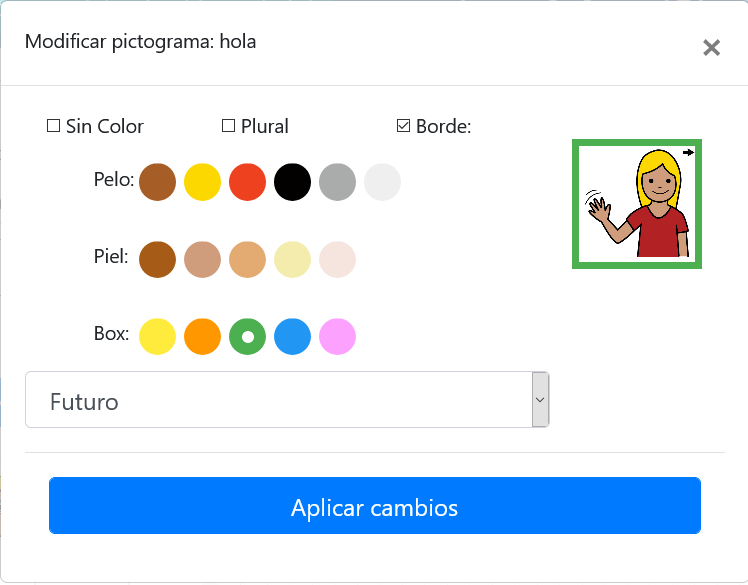
\includegraphics[width=0.7\linewidth]{Imagenes/Bitmap/modalEditarPicto}
	\caption{Vista de la interfaz del modal que muestra una edición de pictogramas con más opciones. En este caso, se ha seleccionado el tiempo futuro y el borde verde. }
	\label{fig:modaleditarpicto}
\end{figure}


\subsubsection{Reproducir sonido}


La función del botón es la de reproducir mediante audio el nombre del pictograma. Como se ha visto anteriormente, los pictogramas devueltos por la API pueden contar con locución si se consulta el parámetro “\textit{hasLocution}”. En caso de contar con locución, se accede a la URL\footnote{\url{https://privateapi.arasaac.org/api/locutions/es/}} que contiene la pista de voz asociada y se reproduce. 
En caso de no contar con locución se ha usado \textit{SpeechSynthesisUtterance}\footnote{\url{https://developer.mozilla.org/en-US/docs/Web/API/SpeechSynthesisUtterance}} para que haga una función similar en el resto de pictogramas. Está configurada para que sintetize la voz en español y es compatible con todos los navegadores modernos.

\subsection{Reglas de diseño de usabilidad}
 Las reglas de diseño utilizadas en esta funcionalidad han sido:

\begin{itemize}
	\item \textbf{Coherencia}: esta herramienta hace usos de iconos para ayudar al usuario de una manera visual a saber que acción va a realizar. Los iconos utilizados son: una lupa para realizar la búsqueda, un icono al lado de la lupa para ver el historial de búsqueda y unos engranajes en la parte de la derecha para realizar el preajuste de los pictogramas.
	
	También se utilizan los iconos de “+” para añadir el pictograma al tablero y el icono de la carpeta para añadir el pictograma a una nueva lista o a una ya creada.
	
	En PictoItem también se utilizan iconos que representarán distintas funcionalidades sobre el pictograma. Por ejemplo, en la esquina superior derecha hay una “×” para eliminar el pictograma y en la parte inferior iconos de un lápiz para editar el pictograma y un icono de un triángulo para reproducir la palabra. Algunos iconos como la “×” o el icono del lápiz también será utilizados por otros ítems y estarán en las mismas posiciones y harán funciones similares. Esto se hace para crear uniformidad y ayudar al usuario a familiarizarse con la aplicación.
	
	
	\item \textbf{Usabilidad universal}: el principio de usabilidad reconoce las necesidades de los distintos tipos de usuarios ya sean nuevos o expertos en la aplicación. Esto queda reflejado en el apartado de búsqueda de pictogramas con la opción de preajuste de pictogramas. Por ejemplo, un usuario en la aplicación añadiría un pictograma al tablero y después lo editaría, pero mediante el preajuste permite añadir varios pictogramas sin tener que editarlos individualmente.
	
	\item \textbf{Retroalimentación informativa}: el usuario, tras realizar la búsqueda, verá visualmente todos los pictogramas cuyo significado coincide con la palabra a buscar. También tras pulsar el botón “+” sobre un pictograma, este automáticamente se añadirá al tablero.
	
	
	\item \textbf{Permitir deshacer acciones de forma fácil}: en caso de escribir mal la palabra al realizar la búsqueda el usuario podrá borrarla y volver a escribirla correctamente para buscar los pictogramas que correspondan con esa palabra.
\end{itemize}


\section{Traducir frase a pictogramas}
\label{cap5:sec:traduccion}
La herramienta de traducción de frase a pictograma se encuentra en la segunda pestaña que agrupa las herramientas para añadir pictogramas e imágenes, tal y como se puede ver en la Figura \ref{fig:traducirfraseinicial}. Cuenta con un ítem propio llamado FraseItem, que agrupa los pictogramas de la traducción para ser desplazados en bloque por la cuadrícula.

La traducción de frase a pictogramas, como su nombre indica, ofrece una interfaz que permite al usuario escribir una frase y recibir la traducción en pictogramas. Nuevamente, en la Figura \ref{fig:traducirfraseinicial} se puede ver la interfaz inicial de la traducción a frase, muy similar a la vista en la búsqueda de picto en la Figura \ref{fig:buscarpicto2}. 

% TODO: \usepackage{graphicx} required
\begin{figure}[h!]
	\centering
	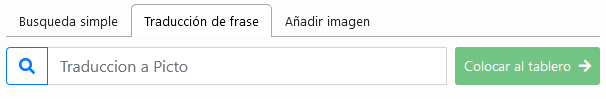
\includegraphics[width=0.7\linewidth]{Imagenes/Bitmap/traducirFraseInicial}
	\caption{Interfaz inicial Traducción frase a pictograma.}
	\label{fig:traducirfraseinicial}
\end{figure}

 
La traducción es realizada mediante la API de ARASAAC. Aunque no cuenta con una traducción dedicada a frases, se traduce el texto palabra a palabra de la frase escrita. Por cada palabra se realizará una búsqueda que devolverá entre 0 o más pictogramas. Inicialmente la traducción se iba a realizar mediante la API de accesibilidad del grupo NIL, que cuenta con una función dedicada a la traducción de frases a pictogramas. En la Sección \ref{cap5:sec:nilgroup} se explicará por qué no ha sido utilizada. 


El resultado de la traducción no está fijado a un pictograma concreto por palabra, sino que puede haber varios. Es por ello que se devuelven de un modo u otro varios pictogramas posibles por cada palabra de la frase.  En la Figura \ref{fig:traduccionpicto} se puede ver cómo la interfaz permite navegar entre los pictogramas alternativos mediante dos botones.
Estos botones permiten avanzar y retroceder entre los pictogramas alternativos que se muestran por cada palabra. Por último, destacar que el botón “Colocar al tablero” no se activa hasta que no hay una frase traducida, como se puede ver en las Figuras \ref{fig:traducirfraseinicial} y \ref{fig:traduccionpicto}. 

% TODO: \usepackage{graphicx} required
\begin{figure}[h!]
	\centering
	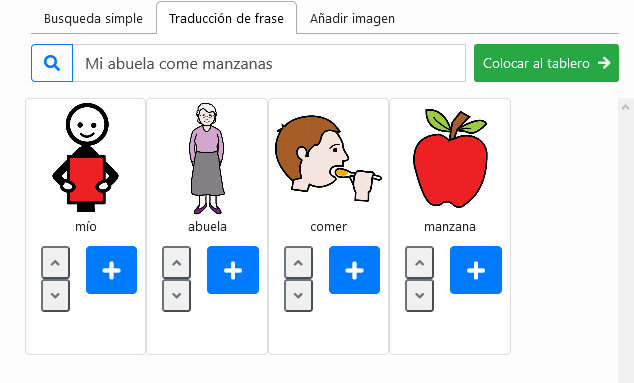
\includegraphics[width=0.7\linewidth]{Imagenes/Bitmap/traduccionPicto}
	\caption{Resultado de la traducción de una frase.}
	\label{fig:traduccionpicto}
\end{figure}

El componente también permite añadir los pictogramas de manera individual al pulsar sobre el botón “+”, tal y como sucedía en búsqueda de pictograma. En caso de que se pulse sobre “Colocar al tablero”, se colocarán en el tablero todos los pictogramas juntos en un único elemento FraseItem. 

\subsection{FraseItem}

Como se puede ver en la Figura \ref{fig:fraseitemoriginal} este tipo de  ítem agrupa todos los pictogramas recibidos de la traducción. De esta manera el usuario, para desplazarlo por el tablero, no tiene que mover cada pictograma de manera individual. Este ítem cuenta además con la posibilidad de ocultar pictogramas ya que el usuario podría no querer que se muestre alguno. Para ello se ha de presionar en el botón de edición con el icono del lápiz. 

% TODO: \usepackage{graphicx} required
\begin{figure}[h!]
	\centering
	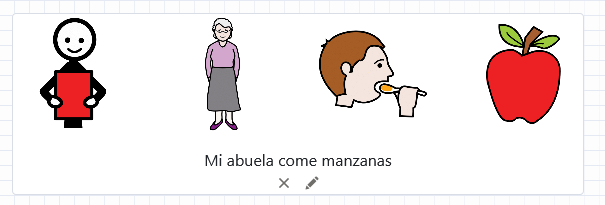
\includegraphics[width=0.7\linewidth]{Imagenes/Bitmap/fraseItemOriginal}
	\caption{Vista de FraseItem en la cuadrícula.}
	\label{fig:fraseitemoriginal}
\end{figure}


Al ser presionado aparecerá un nuevo modal como se ve en la Figura \ref{fig:modaleditarfraseitem}. Está compuesto por una previsualización de la frase en la parte superior, y en la parte inferior los pictogramas que componen la frase junto al botón que permite esconderlos o mostrarlos. Dicho botón cambiará de apariencia según el estado de visualización del pictograma. Si es visible el botón representa un ojo en azul, y en caso contrario se representará mediante un ojo tachado en rojo ocultando el pictograma de la previsialización superior. Al presionar alguno de ellos, se actualiza la previsualización. Por último, debajo existe un campo de texto donde se puede editar el contenido de la frase.
En la Figura \ref{fig:fraseitemmidificada} se puede ver un ejemplo de cómo quedaría el ítem tras aplicar los cambios. 

% TODO: \usepackage{graphicx} required
\begin{figure}[h!]
	\centering
	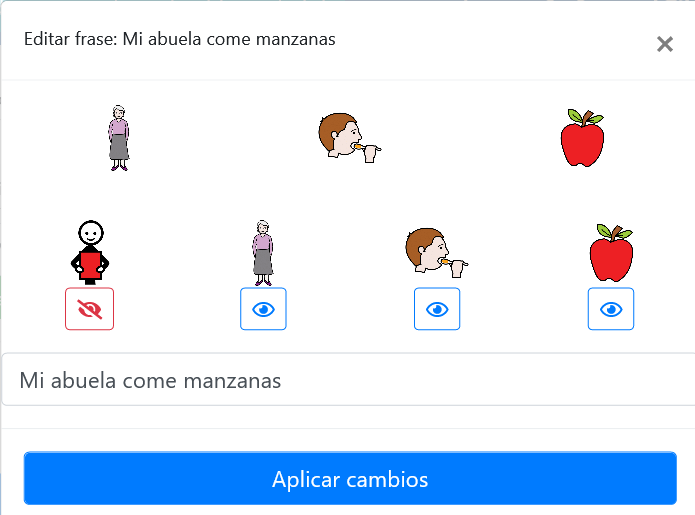
\includegraphics[width=0.7\linewidth]{Imagenes/Bitmap/modalEditarFraseItem}
	\caption{Vista del modal de edición del FraseItem.}
	\label{fig:modaleditarfraseitem}
\end{figure}

% TODO: \usepackage{graphicx} required
\begin{figure}[h!]
	\centering
	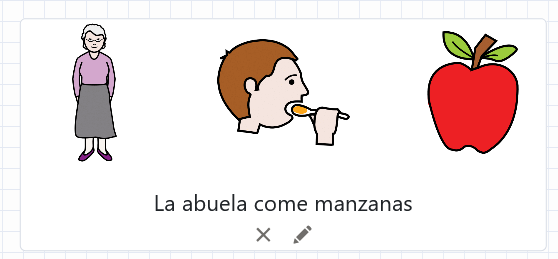
\includegraphics[width=0.7\linewidth]{Imagenes/Bitmap/fraseItemMidificada}
	\caption{FraseItem tras  aplicar los cambios.}
	\label{fig:fraseitemmidificada}
\end{figure}

\subsection{Reglas de diseño de usabilidad}
\label{cap5:reglasBusqueda}
 Las reglas de diseño utilizadas en esta funcionalidad han sido:
 
\begin{itemize}
	\item \textbf{Coherencia}: al igual que en el buscador de pictogramas se utiliza el icono de la lupa para realizar la traducción de la frase. También se utilizan unas flechas como iconos para ver todos los pictogramas asociados a cada palabra, y al igual que en el buscador de pictogramas se incluye el icono “+” para añadir individualmente un pictograma.
	
	\item \textbf{Retroalimentación informativa}: tras pulsar el botón para realizar la traducción de la frase se le mostrará al usuario todos los pictogramas asociados a las palabras de la frase.  También si el usuario pulsa sobre las flechas de un pictograma se le mostrará otros pictogramas con un significado similar permitiendo así escoger el que más le guste al usuario. Por último, tras haber realizado una traducción de una frase y al pulsar sobre el botón para colocarla en el tablero, la frase se añadirá al tablero informando de esta manera que la acción se ha realizado correctamente.
	
	\item \textbf{Prevenir errores}: para evitar que el usuario añada una frase vacía al tablero, el botón de “Colocar al tablero” se habilitará cuando se haya realizado una traducción. Tras borrar la frase en el campo de texto el botón se volverá a deshabilitar.
	
	
	\item \textbf{Permitir deshacer acciones de forma fácil}: si el usuario escribe mal la frase a traducir siempre podrá corregir los errores de escritura y realizar la traducción de la frase. También podrá eliminar la fraseItem del tablero pulsando sobre el icono “+” de su interior.
	
\end{itemize}





\section{Añadir imagen al tablero}
\label{cap5:sec:imagen}
Añadir una imagen al tablero se encuentra en la tercera pestaña que agrupa todas las herramientas que añaden pictogramas o fotos a la cuadrícula. Como se puede ver en la Figura \ref{fig:cargarfotopestana}, su interfaz inicial consiste en un simple botón que carga una imagen del explorador de archivos del dispositivo. Está especificado que solo acepte archivos de tipo imagen, previniendo así posibles errores del usuario. 

% TODO: \usepackage{graphicx} required
\begin{figure}[h!]
	\centering
	\includegraphics[width=0.7\linewidth]{Imagenes/Bitmap/cargarFotoPestaña}
	\caption{Interfaz inicial al añadir una imagen al tablero.}
	\label{fig:cargarfotopestana}
\end{figure}


Al cargar la imagen correctamente, tal y como se puede ver en la Figura \ref{fig:addphotoitem}, se mostrará: 

\begin{itemize}
	\item Una previsualización de la imagen.
	\item Un campo de texto para añadirlo debajo de la imagen.
	\item Un botón para añadir la imagen a la cuadrícula.
\end{itemize}

% TODO: \usepackage{graphicx} required
\begin{figure}[h!]
	\centering
	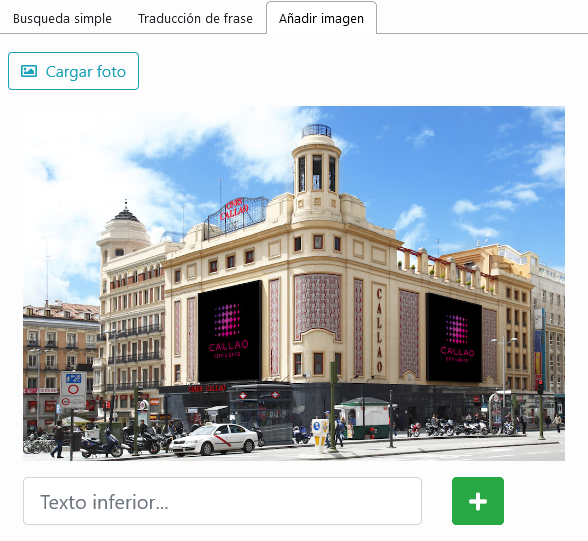
\includegraphics[width=0.7\linewidth]{Imagenes/Bitmap/addPhotoItem}
	\caption{ Vista de la Interfaz al cargar una imagen.}
	\label{fig:addphotoitem}
\end{figure}



Al presionar el botón de añadir, antes de enviar la información de la foto, se obtiene su valor de alto y ancho en píxeles. Estos datos serán utilizados para conocer la proporción de la imagen. Respecto al acceso a los datos de la foto, se realiza por una URL que funciona únicamente en la sesión vigente generada mediante \texttt{URL.createObjectURL}\footnote{\url{https://developer.mozilla.org/en-US/docs/Web/API/URL/createObjectURL}}.

Al enviar la información de la foto a la capa superior se envían los siguientes parámetros: 

\begin{itemize}
	\item URL de la imagen.
	\item Ancho y alto en píxeles.
	\item Texto inferior. En caso de no haber sido escrito nada, se enviará vacío.
\end{itemize}

Se estudiaron otras maneras de cargar las imágenes, como importarlas desde Google Drive o un archivo zip. Sin embargo fueron descartadas. En la Sección \ref{cap5:addImageCut} se especificarán los motivos. 

\subsection{PhotoItem}

Su representación en el tablero es la imagen dentro del ítem. El ancho y alto del ítem es proporcional a la imagen original, como se calculó anteriormente. 

Respecto al texto inferior, se puede ver en la Figura \ref{fig:photoitemtexto} que puede aparecer o no. Si se ha recibido un texto inferior, éste aparecerá en un espacio reservado para él debajo de la imagen. En caso contrario la imagen abarcará la totalidad del ítem.

% TODO: \usepackage{graphicx} required
\begin{figure}[h!]
	\centering
	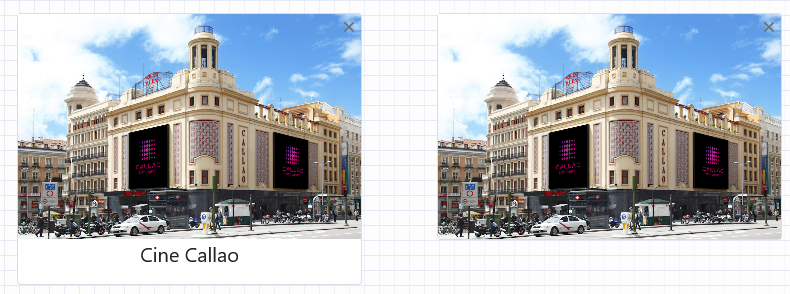
\includegraphics[width=0.7\linewidth]{Imagenes/Bitmap/photoItemTexto}
	\caption{Ejemplod de PhotoItem con y sin texto.}
	\label{fig:photoitemtexto}
\end{figure}


En la Figura \ref{fig:photoitemerror} se ejemplifica qué pasaría si en vez de calcular la proporción de la imagen, se dejara siempre con un ancho y alto fijo apareciendo espacios en blanco.

% TODO: \usepackage{graphicx} required
\begin{figure}[h!]
	\centering
	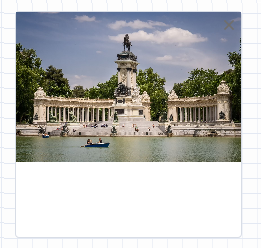
\includegraphics[width=0.7\linewidth]{Imagenes/Bitmap/photoItemError}
	\caption{Ejemplo de PhotoItemn si no se mantuviera la proporción según el tamaño de la imagen.}
	\label{fig:photoitemerror}
\end{figure}

\subsection{Reglas de diseño de usabilidad}

 Las reglas de diseño utilizadas en esta funcionalidad han sido:
\begin{itemize}
	\item \textbf{Coherencia}: como en las otras herramientas, se hace uso de iconos para proporcionar al usuario una manera más simple y visual de la acción va a realizar. Un ejemplo de icono utilizado es el botón con el “+” para añadir la imagen al tablero. Al igual que en otros items como PictoItem o FraseItem el componente PhotoItem también tiene un icono “×” para poder ser eliminado del tablero.
	
	\item \textbf{Retroalimentación informativa}: tras pulsar sobre el botón “Cargar foto” y seleccionar una imagen, se mostrará en la parte de abajo una previsualización de la imagen. Esto permite al usuario ver si la imagen seleccionada es la correcta.
	También podemos ver que esta regla se cumple al pulsar sobre el botón con el icono “+”, el cual añadirá al tablero la imagen seleccionada.
	
	
	\item \textbf{Permitir deshacer acciones de forma fácil}:  tras cargar una imagen y no ser la deseada por el usuario, este podrá volver a seleccionar una nueva imagen que posteriormente se previsualizará. También se podrá eliminar un PhotoItem que ya esté añadido en el tablero pulsado sobre el icono “+” de su interior.
	
\end{itemize}



\section{Listas de pictogramas}
\label{listapictos}

Esta herramienta permite crear distintas listas donde el usuario podrá añadir los pictogramas que desee.
Para implementar esta herramienta se necesita tener una estructura donde se guarde el nombre de cada una de las listas y todos los elementos PictoItem que contenga. 

\subsection{Añadir y crear a una lista}

Para crear una lista o añadir un pictograma a una lista existente, el usuario deberá pulsar sobre el icono de la carpeta de un pictograma tras realizar una búsqueda, tal y como se puede ver en la Figura \ref{fig:buscarpicto2}. Tras pulsar el icono se desplegará un modal donde dependiendo del estado de las listas mostrará un menú u otro. En el caso de que no haya ninguna lista simplemente se mostrará la opción de crear una lista donde se deberá introducir el nombre de la lista a crear, mientras que si ya había alguna lista creada se mostrará un menú con la posibilidad de añadir el pictograma seleccionado a una lista existente o crear una nueva lista. Un ejemplo de esto lo podemos ver en la Figura \ref{fig:modalescoleccion} donde el modal de la izquierda aparece cuando no existe ninguna lista y el de la derecha cuando ya existe al menos una lista. Además la lista mostrada en el modal de la izquierda será la última lista modificada.


% TODO: \usepackage{graphicx} required
\begin{figure}[h!]
	\centering
	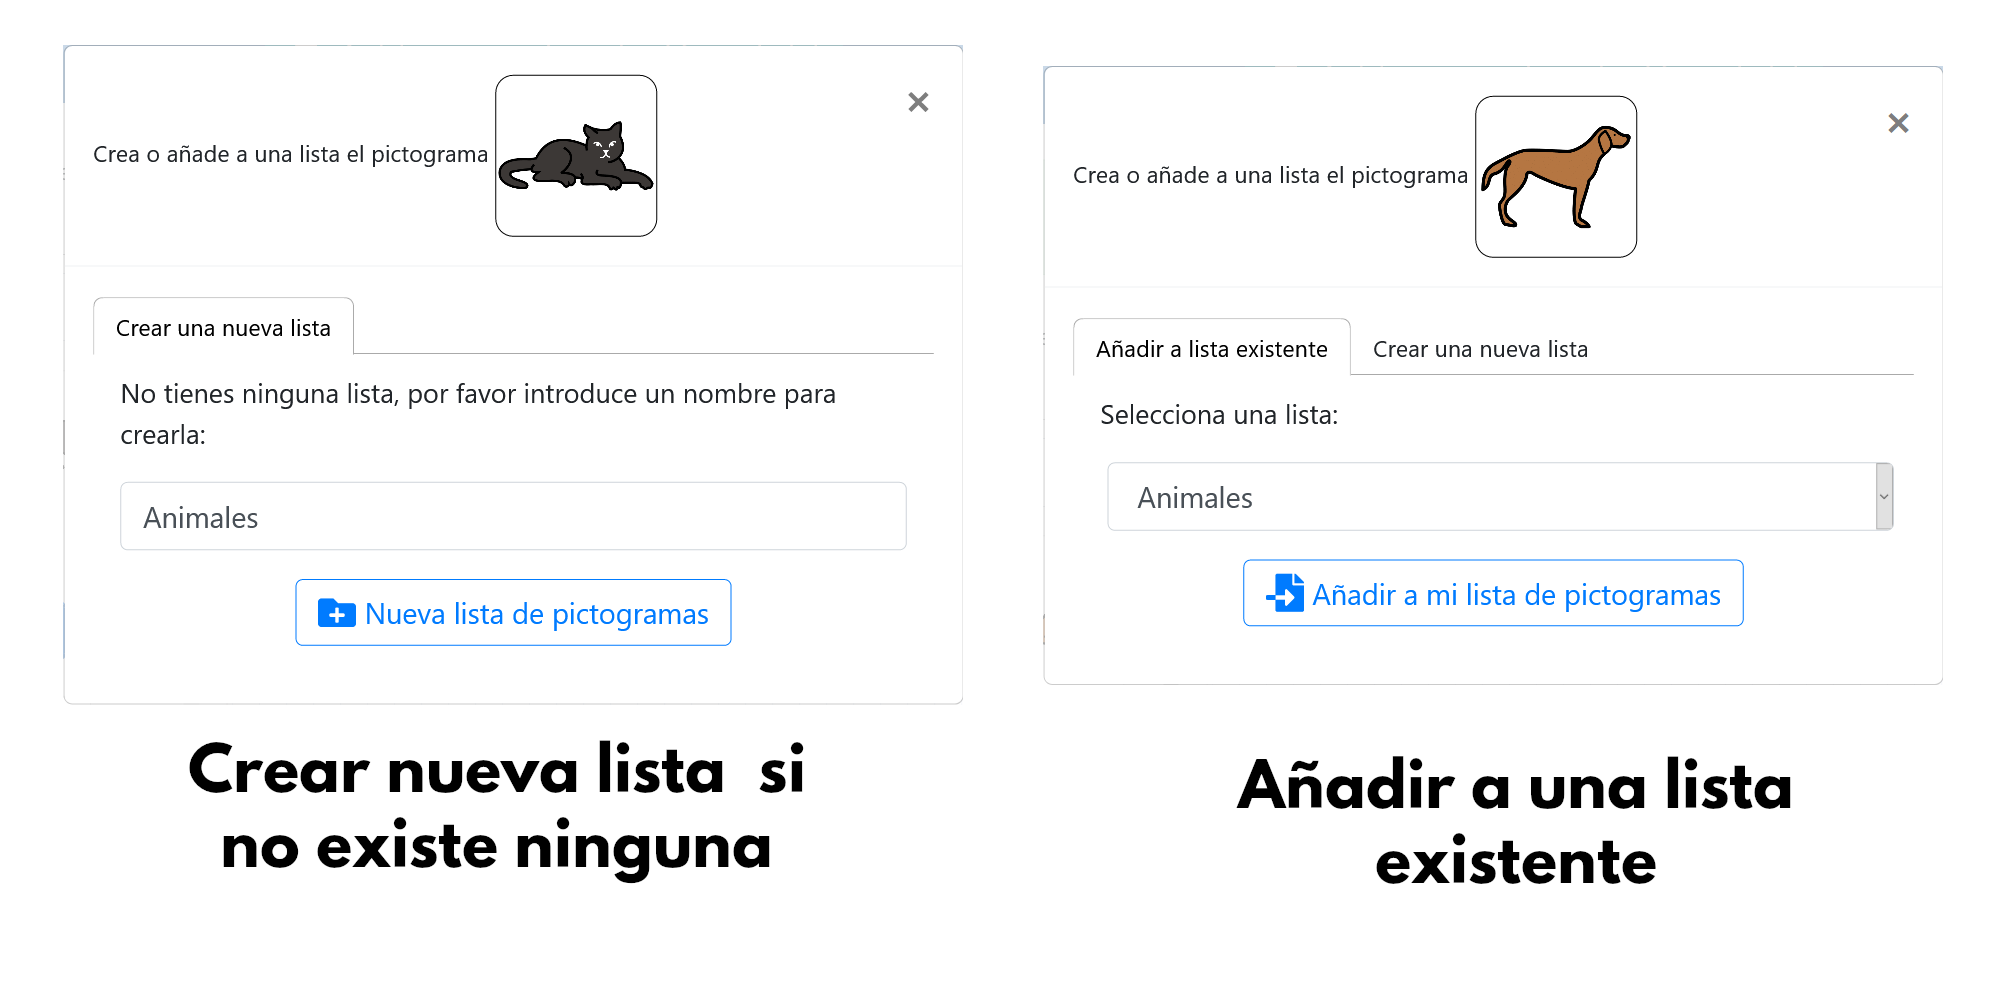
\includegraphics[width=0.7\linewidth]{Imagenes/Bitmap/modalesColeccion}
	\caption{Vistas del modal con ninguna lista y al menos una, respectivamente.}
	\label{fig:modalescoleccion}
\end{figure}


Para informar al usuario de las acciones, tanto la de crear una nueva lista, como añadir un pictograma a una lista existente se han utilizado alertas (mensajes). Estas alertas a parte de dar una cierta información al usuario también sirven para tener un cierto control de errores para que el usuario no cree dos listas con el mismo nombre o que no añada un pictograma dos veces a una lista.


\begin{itemize}
	\item En el caso de que se haya podido realizar la acción con éxito se mostrará un pequeño mensaje descriptivo de la acción en verde (Figura \ref{fig:alertlistapicto}).
	
	% TODO: \usepackage{graphicx} required
	\begin{figure}[h!]
		\centering
		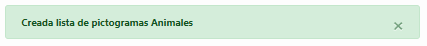
\includegraphics[width=0.7\linewidth]{Imagenes/Bitmap/alertListaPicto}
		\caption{Alerta tras añadir satisfactoriamente un pictograma a la lista.}
		\label{fig:alertlistapicto}
	\end{figure}
	
	
	\item  En el caso de que la acción no se haya podido realizar correctamente se informará al usuario con un mensaje en rojo, como el que se ve en la Figura \ref{fig:alerterrorlistapicto}, informando al usuario el por qué no ha podido realizarla.
	
	% TODO: \usepackage{graphicx} required
	\begin{figure}[h!]
		\centering
		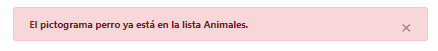
\includegraphics[width=0.7\linewidth]{Imagenes/Bitmap/alertErrorListaPicto}
		\caption{Alerta de acción no permitida.}
		\label{fig:alerterrorlistapicto}
	\end{figure}
	
	
	
\end{itemize}

\subsection{Gestión de listas de pictogramas}

Otras funcionalidades que podemos encontrar en esta herramienta es la posibilidad de importar y exportar las listas creadas.
Para la funcionalidad de exportar guardaremos el estado actual de las listas en un fichero con extensión “.json”. Para la generación de este documento se utilizará la función \textit{JSON.stringify()}, la cual nos permitirá crear la estructura propia de los json y posteriormente generar el documento con ese contenido.

La funcionalidad de importar cargará el estado de las listas a partir del archivo creado anteriormente. Para ello se hará uso de la función \textit{JSON.parse()}, la cual convertirá el json a la estructura de listas requerida. En caso de ya existir listas en la aplicación, las nuevas listas cargadas se añadirán a las ya existentes. 

Por último, las listas existentes se encuentran en el apartado “Mis listas de pictogramas”, como se muestra en la Figura \ref{fig:lisapictosel}. Para visualizar una de ellas deberemos seleccionar el nombre de esta de entre todas las disponibles. A continuación, al igual que en el apartado de búsqueda de pictograma, se mostrarán todos los pictogramas con su imagen, texto correspondiente y el botón de “+” que permite añadirlo a la cuadrícula como un PictoItem visto anteriormente.

% TODO: \usepackage{graphicx} required
\begin{figure}[h!]
	\centering
	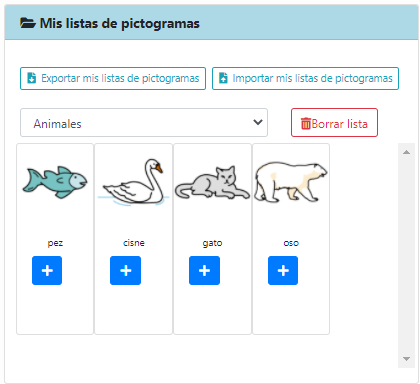
\includegraphics[width=0.7\linewidth]{Imagenes/Bitmap/lisaPictoSel}
	\caption{Vista de las listas de pictogramas.}
	\label{fig:lisapictosel}
\end{figure}

\subsection{Reglas de diseño de usabilidad}

Las reglas de diseño utilizadas en esta funcionalidad han sido:
\begin{itemize}
	\item \textbf{Coherencia}: se ha utilizado el icono de una carpeta para todas las acciones que tiene que ver con las listas de pictogramas. Este icono aparece tanto en los pictogramas devueltos tras realizar una búsqueda simple como en el apartado “Mis listas de pictogramas”.  También se utilizan iconos similares en los botones de los modales, como por ejemplo en el botón para añadir una nueva lista cuyo icono es una carpeta con un más dentro, o en el apartado añadir a una lista existente donde el icono es una flecha señalando a un documento, haciendo alusión a que se va a incluir en la lista indicada previamente.
	
	\item \textbf{Retroalimentación informativa}: para informar al usuario de si una acción se ha podido realizar correctamente o no se han utilizado las alertas. Las alertas utilizadas pueden ser de dos tipos: verdes para las acciones realizadas correctamente y las rojas para las acciones que han dado algún tipo de error como crear dos listas con el mismo nombre. Éstas aparecen siempre en la parte superior de la pantalla junto con un texto descriptivo de la acción que se ha realizado para asegurar que sean vistas con facilidad.
	
	\item \textbf{Prevenir errores}: la aplicación está diseñada para prevenir que el usuario cometa un error y en caso de error sea detectado e informe con un breve mensaje describiéndolo. Este tipo de patrón se aplica en todas las acciones correspondientes a las listas de pictogramas a la hora de crear una lista, donde se comprueba que la lista tenga un nombre y no se repita con otra existente, y al añadir un pictograma a una lista donde se verifica que no se haya añadido anteriormente. En caso de error se utilizarán las alertas con un mensaje informando del problema.
	
	
	\item \textbf{Permitir deshacer acciones de forma fácil}: en caso de que el usuario cree una lista por error la podrá borrar desde el apartado “Mis listas de pictogramas” donde deberá seleccionar la lista creada y pulsar sobre el botón de borrar lista.
	
\end{itemize}


\section{Texto}

Esta herramienta permite añadir un cuadro de texto a la cuadrícula. Como opciones de personalización de texto se ofrece la posibilidad al usuario de seleccionar una tipografía entre las seis posibles. Las tipografías elegidas son las más utilizadas dentro del ámbito educativo, se pueden ver algunos ejemplos de ellas en la Figura \ref{fig:fraseitem1}.

Esta herramienta se puede encontrar en el apartado de “Personalización de tablero”, donde se podrán seleccionar distintas tipografías y escribir el texto que se va a añadir a la cuadrícula.

Como se puede ver en la Figura \ref{fig:anadirtexto} en la parte superior se puede elegir una tipografía y a su derecha ver una previsualización de ésta. Debajo, está el campo de texto donde se escribirá la frase seguido del botón para añadirla a la cuadrícula.

% TODO: \usepackage{graphicx} required
\begin{figure}[h!]
	\centering
	\includegraphics[width=0.7\linewidth]{Imagenes/Bitmap/añadirTexto}
	\caption{Vista de la selección de fuente y campo de texto.}
	\label{fig:anadirtexto}
\end{figure}


Para poder implementar este componente, en su estructura se guardará el texto que se vaya a añadir a la cuadrícula y la tipografía seleccionada.

A diferencia de otros elementos como los pictogramas en los que el ancho y alto del ítem era proporcional, en el texto se permite ajustar ambas propiedades de manera independiente.

\subsection{TextoItem}
\label{cap5:sec:texto}
Al añadir el texto a la cuadrícula, el ancho del ítem se ajustará al número de caracteres del texto. En la parte inferior del ítem como se ve en la Figura \ref{fig:fraseitem1} se encuentran tres botones, dos para reducir y aumentar el tamaño de la fuente del texto y otro para editar su contenido.

% TODO: \usepackage{graphicx} required
\begin{figure}[h!]
	\centering
	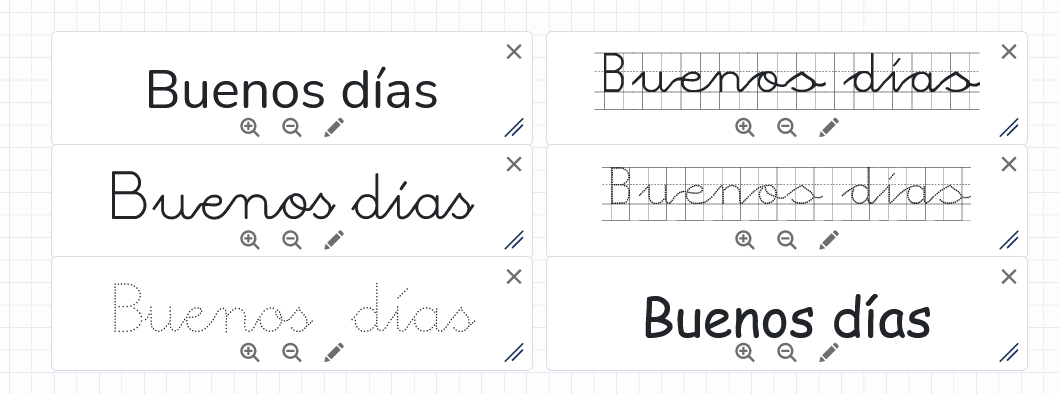
\includegraphics[width=\linewidth]{Imagenes/Bitmap/fraseItem1}
	\caption{Representación del TextoItem en la cuadrícula con las distintas tipografías disponibles.}
	\label{fig:fraseitem1}
\end{figure}


Al pulsar sobre el icono del lápiz se desplegará el modal de edición de ítem. Como se ve en la Figura \ref{fig:modaleditartexto}, cuenta con un campo donde se puede ver y editar el contenido actual del texto. Esto resultará muy útil para corregir errores ortográficos. Tras pulsar sobre el botón “Cambiar texto”, el ancho del ítem se ajustará de nuevo en función del nuevo número de caracteres.

% TODO: \usepackage{graphicx} required
\begin{figure}[h!]
	\centering
	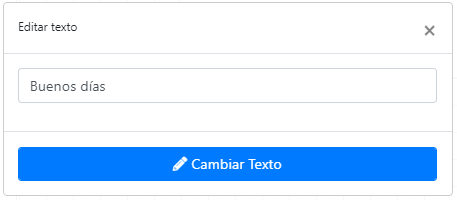
\includegraphics[width=0.7\linewidth]{Imagenes/Bitmap/modalEditarTexto}
	\caption{Vista del modal para editar un TextoItem.}
	\label{fig:modaleditartexto}
\end{figure}

\subsection{Reglas de diseño de usabilidad}

 Las reglas de diseño utilizadas en esta funcionalidad han sido:
\begin{itemize}
	\item \textbf{Coherencia}:  un TextoItem añadido al tablero contará con múltiples botones, en la parte superior derecha tendrá una “×” para eliminar el texto del tablero y en la parte inferior dos iconos de unas lupas para ampliar o reducir la fuente del texto y un icono de un lápiz para poder editar el contenido.
	
	\item \textbf{Retroalimentación informativa}: en el apartado de “Personalización del tablero” el usuario podrá seleccionar distintos tipos de fuentes de letras donde verá al instante un ejemplo de la fuente seleccionada. Además, cuando el usuario pulse sobre el botón de “+Texto” verá de manera instantánea el texto en el tablero de la aplicación. De esta manera se le informa al usuario de que la acción se ha realizado correctamente. También afecta a la acción de borrar el texto del tablero, ya que cuando el usuario pulse sobre el icono “×” automáticamente se borrará del tablero.
	
	
	\item \textbf{Permitir deshacer acciones de forma fácil}: en caso de haber añadido el texto al tablero con una falta de ortografía el usuario podrá editar el contenido del TextoItem pulsando sobre el icono del lápiz. También podrá eliminar el texto del tablero en caso de que haya sido añadido por error, para esto deberá pulsar sobre el icono “×” situado en la esquina superior derecha.
	
\end{itemize}



\section{Iconos}
\label{cap5:sec:iconos}
El componente icono permite añadir a la cuadrícula iconos y personalizarlos. Los iconos disponibles son: cuadrado, tick, barra y corazón, como se muestra en la Figura \ref{fig:herramientaitems}. El componente está formada por una estructura donde se guarda el tipo de icono, el color y la opacidad.

% TODO: \usepackage{graphicx} required
\begin{figure}[h!]
	\centering
	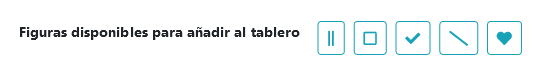
\includegraphics[width=0.7\linewidth]{Imagenes/Bitmap/herramientaItems}
	\caption{Vista de los botones que añaden iconos.}
	\label{fig:herramientaitems}
\end{figure}


A la hora de mostrar los iconos en la cuadrícula hay que hacer una distinción entre el cuadrado y el resto de los iconos ya que la forma en la que se muestran es distinta.

Para generar un cuadrado se hace uso de las formas geométricas básicas que ya están implementadas en \textit{SVG}. Este lenguaje de marcas permite crear figuras geométricas y personalizar su aspecto. Para representar el cuadrado se ha de incluir la etiqueta \textit{<rect/>} (etiqueta para generar un cuadrado) y añadir las propiedades que queremos que tenga como por ejemplo altura, ancho, grosor de los bordes del cuadrado, color u opacidad.

Sin embargo, para el resto de los iconos se utilizan recursos obtenidos de FontAwesome\footnote{\url{https://fontawesome.com/}}. Este framework tiene implementado iconos vectoriales que al igual que con el cuadrado, permiten la personalización de los iconos respecto a el color, tamaño y opacidad. Para mostrarlos se deberá incluir la clase correspondiente de cada icono especificada en el apartado tipo de la estructura.

En la Figura \ref{fig:ejemplopictoitem} se puede ver que estos iconos se pueden superponer a los pictogramas para realzar ideas. Aunque la forma de visualizarlos se hace de manera distinta dependiendo del icono, todos ellos permiten editar ciertos aspectos. Es por ello por lo que se incluyó la funcionalidad de editar. Para poder editar un icono añadido a la cuadrícula tendremos que pulsar sobre el icono del lápiz, al pulsarlo aparecerá un modal, como el de la Figura \ref{fig:modalpictoitem} donde se podrá modificar el color y la opacidad del icono. 

% TODO: \usepackage{graphicx} required
\begin{figure}[h!]
	\centering
	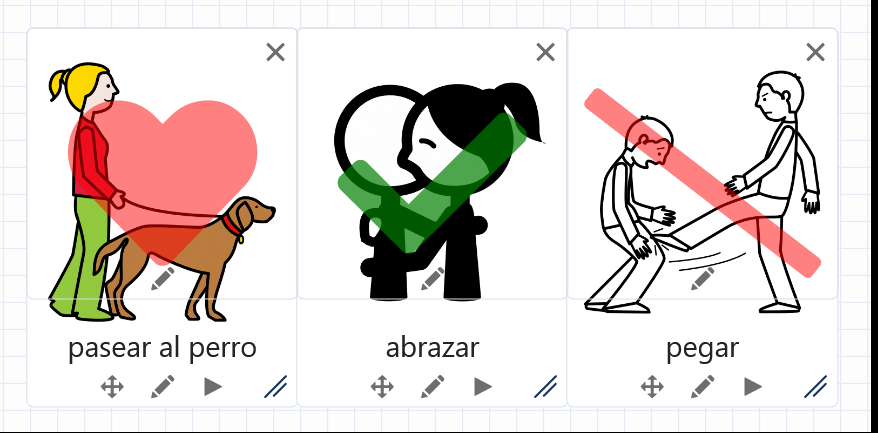
\includegraphics[width=0.7\linewidth]{Imagenes/Bitmap/ejemploPictoItem}
	\caption{Ejemplo de uso de iconos sobre algunos pictogramas.}
	\label{fig:ejemplopictoitem}
\end{figure}

% TODO: \usepackage{graphicx} required
\begin{figure}[h!]
	\centering
	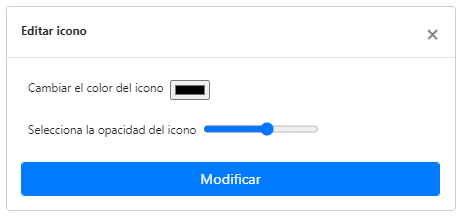
\includegraphics[width=0.7\linewidth]{Imagenes/Bitmap/modalPictoItem}
	\caption{Vista del modal de edición de iconos.}
	\label{fig:modalpictoitem}
\end{figure}

\subsection{IconoItem}

Cuando un icono se añade al tablero de la aplicación este tendrá una opacidad y color por defecto. A los iconos corazón y barra tendrá por defecto el color rojo y una opacidad al 50\%, y el icono del tick tiene como color por defecto será el verde y una opacidad del 50\%. El hecho de que los iconos tengan por defecto esa opacidad es debido a que están planteados para estar superpuestos encima de los pictogramas, por lo que han de ser translúcidos para ver el pictograma que se encuentra debajo del icono. Por último, el icono del cuadrado por defecto será negro y la opacidad del 100\% ya que están planteados para ser opacos.

En el IconoItem se incluyen dos botones, una “×” en la esquina superior derecha que sirve para eliminar el icono del tablero y un icono de un lápiz en la parte inferior que permite editar el icono. Para poder editar un icono añadido a la cuadrícula tendremos que pulsar sobre el icono del lápiz, al pulsarlo aparecerá un modal, como el de la Figura \ref{fig:modalpictoitem} donde se podrá modificar el color y la opacidad del icono.

\subsection{Reglas de diseño de usabilidad}
 Las reglas de diseño utilizadas en esta funcionalidad han sido:
\begin{itemize}
	\item \textbf{Coherencia}: en el apartado “Personalización del tablero” se muestran todos los iconos disponibles que se pueden añadir al tablero, permitiendo de esta manera mostrar al usuario como son esos iconos antes de ser añadidos. El IconoItem cuenta con un botón en la esquina superior derecha para eliminarlo y un botón con el icono de un lápiz para poder editarlo, al igual que otros items.
	
	
	\item \textbf{Retroalimentación informativa}: al pulsar sobre uno de los botones con iconos en el apartado “Personalización del tablero” automáticamente se añadirá al tablero. De esta manera se informa al usuario de que la acción para añadir un icono se ha realizado correctamente. Para la acción contraria de eliminar un IconoItem simplemente se eliminará del tablero dando a entender al usuario que el icono se ha podido eliminar correctamente. Otra acción que se ve reflejada en esta regla es que tras editar un icono y cerrar el modal, se le asignará al icono el nuevo color y opacidad visualizando el nuevo resultado al instante.
	
	
	\item \textbf{Permitir deshacer acciones de forma fácil}: en caso de añadir un icono por error el usuario podrá eliminarlo desde el tablero. También se permite al usuario volver a cambiar el color o la opacidad de un icono las veces que desee.
	
\end{itemize}


\section{Descargar Tablero}
\label{cap5:descargar}

Esta herramienta permite descargar la cuadrícula como imagen. Para ello se utiliza la librería html2tocanvas\footnote{\url{https://html2canvas.hertzen.com/}}. Ésta librería además permite seleccionar la calidad de descarga de la imagen. Por ello que se ha creado un modal como se puede ver en la Figura \ref{fig:modaldescargartablero} donde el usuario puede elegir la calidad deseada, siendo la calidad alta la elegida por defecto. 

Inicialmente se planteó la posibilidad de descargar estos tableros como PDF pero esta opción no se implementó por falta de tiempo.

% TODO: \usepackage{graphicx} required
\begin{figure}[h!]
	\centering
	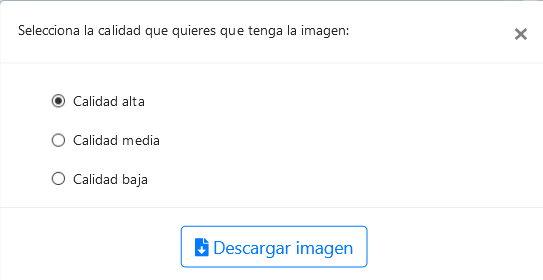
\includegraphics[width=\linewidth]{Imagenes/Bitmap/modalDescargarTablero}
	\caption{Vista del modal para descargar tablero.}
	\label{fig:modaldescargartablero}
\end{figure}



\section{Funcionalidades no implementadas}
\label{cap5:noimplementadas}

Durante el desarrollo de PictUp! se abandonaron algunas funcionalidades debido principalmente a la falta de tiempo o problemas con su integración en la aplicación. A continuación se detallarán los problemas surgidos por cada funcionalidad. 


\subsection{Traducción de frase}
Se trata de la funcionalidad más problemática pues se invirtieron varias semanas en solventarla sin éxito. Una prioridad era la utilización de la NIL-WS-API, pues ofrece una traducciones muy acertadas. A continuación se explicarán los distintos problemas que surgieron durante su implementación.  

\label{cap5:sec:nilgroup}

NIL Web Service\footnote{\url{https://holstein.fdi.ucm.es/nil-ws-api/}} es una API que devuelve información relativa a palabras y textos orientada a resolver problemas de accesibilidad a través del lenguaje. Respecto al tratamiento de palabras, permite buscar sinónimos, antónimos, emociones de las palabras, etc. Para el tratamiento de textos, permite  traducir un texto a pictogramas, listar las emociones de un texto o resumir, entre otras funcionalidades. 

Originalmente la traducción de pictogramas en esta aplicación fue creada específicamente para trabajar con esta API. No obstante también ha causado varios inconvenientes, relativos a los pictogramas que usa la API y los errores causados por \textit{CORS}. 

La API cuenta con una base de datos propia con una gran cantidad de pictogramas. Pero al traducir un texto a pictogramas, esta devuelve por cada palabra o lema, una lista de identificadores. En su mayoría dichos identificadores coinciden con los de los pictogramas de \textit{ARASAAC}, pero existen otros que no. Estos pictogramas que no comparten identificador con los de \textit{ARASAAC} suponen un problema, ya que no se puede obtener toda la información deseada, como por ejemplo el texto, audio y modificaciones. Es por ello que PictoItem se modificó para incluir estos pictogramas suprimiendo la posibilidad de personalizar o reproducir el audio. A continuación se especificará sobre el funcionamiento y problemática asociada a \textit{CORS}.


Cross Origin Resource Sharing\footnote{\url{https://developer.mozilla.org/en-US/docs/Web/HTTP/CORS}}, es un mecanismo de cabeceras http que permite a un servidor dar permiso a otros dominios para cargar recursos del mismo. Por razones de seguridad los navegadores restringen las peticiones de dominio cruzado desde los scripts del navegador. 


Como el servicio de traducción de NIL-WS-API sigue operativo pero descontinuado, no cuenta con la configuración \textit{CORS} y por tanto no puede recibir peticiones \textit{POST} de otras webs. Después de comprender el problema se estudió que la solución es crear un backend para PictUp!. Dicho backend está creado exclusivamente para resolver esta petición. El componente de traducción envía la petición al backend, el cual la resolverá gestionando los \textit{CORS}. En la próxima Sección \ref{backend} se explicará cómo fue creado. 

Después de crear y configurar el backend de manera local, y ver que el componente funcionaba sin complicaciones, apareció otro error con la biblioteca html2canvas\footnote{\url{https://html2canvas.hertzen.com/}}, encargada de crear una imagen a partir de la cuadrícula y sus ítems. Esto es debido a que las imágenes que retorna NIL-WS-API son un recurso externo y la biblioteca htm2canvas desconoce su fuente. Por ello al descargar la imagen del tablero estos pictogramas no aparecían representados dejando un hueco en blanco.


\subsection{Backend}
\label{backend}

El backend fue creado mediante Express\footnote{\url{http://expressjs.com/en/starter/installing.html}}. Se trata de un framework de Node.js que permite gestionar llamadas a API de manera sencilla. Express cuenta con una dependencia que gestiona los \textit{CORS}\footnote{\url{https://www.npmjs.com/package/cors }}, la cual fue usada para realizar el método POST a NIL-WS-API. 

Para esquematizar cómo se obtienen los pictogramas de NIL-WS-API, se puede ver en la Figura \ref{fig:diagramaconexiones} un diagrama de las llamadas que se realizan entre las aplicaciones. 

% TODO: \usepackage{graphicx} required
\begin{figure}[h!]
	\centering
	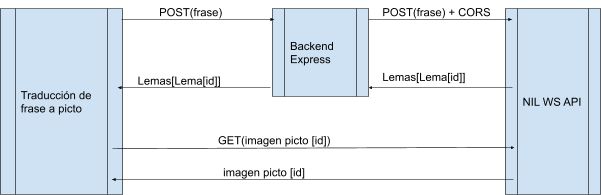
\includegraphics[width=0.7\linewidth]{Imagenes/Bitmap/diagramaConexiones}
	\caption{Diagrama de conexiones entre aplicaciones para traducir una frase.}
	\label{fig:diagramaconexiones}
\end{figure}


Después de varias semanas investigando todos estos problemas, finalmente se detuvo el desarrollo de este componente ya que la fecha para mostrar la web a los usuarios se acercaba. Al tener un prototipo funcional de traducción mediante la API de ARASAAC, aunque asumiendo la baja calidad sintáctica de ésta se consideró suficiente para estudiar la facilidad de uso de la interfaz por parte de los usuarios.




\subsection{Añadir imagen}
\label{cap5:addImageCut}

Originalmente hubo dos aproximaciones sobre la inserción de imágenes. La primera consistía en poder cargar un archivo comprimido \textit{ZIP} mediante la librería JSZip\footnote{\url{https://stuk.github.io/jszip/}} que contaba con funciones para descomprimir archivos. El objetivo era automatizar la colocación de imágenes sobre el tablero, mediante un \textit{ZIP} que almacenara éstas junto a un documento con la información de cada una. Dicho documento incluiría el nombre, la posición y el tamaño de cada imagen colocada en la cuadrícula. Descomprimiendo dicho \textit{ZIP}, las imágenes volverían a ser colocadas a la posición original.

La otra aproximación ofrecía la posibilidad de conectarse mediante la API de Google Drive\footnote{\url{https://developers.google.com/drive/api/v3/about-sdk }} para que el usuario pudiese acceder a sus fotos almacenadas en su cuenta. 

Pese a haber dedicado varias semanas a cada una de estas opciones en proyectos independientes, fueron abandonadas por no obtener resultados satisfactorios. En el caso de JSZip, aunque la compresión de las fotos y descarga del zip funcionara correctamente, surgieron problemas con la librería a la hora de descomprimir los archivos. Respecto a la API de Google Drive, debido a la falta de documentación sobre cómo usarla en React, apenas se logró un prototipo funcional en el tiempo establecido. 

Hubo una última opción que se planteó: realizar un historial de imágenes cargadas muy similar al historial de pictogramas visto anteriormente. Sin embargo, LocalStorage apenas permitía unos pocos megabytes de almacenamiento. La alternativa a LocalStorage fue indexedDB. 

IndexedDB\footnote{\url{https://developer.mozilla.org/en-US/docs/Web/API/IndexedDB_API}} es una API que permite almacenar información en el cliente, en este caso el ordenador del usuario. En ella se pueden crear bases de datos con la capacidad de almacenar archivos de gran tamaño como en este caso imágenes y fotos. Al final fue descartado por falta de tiempo, pero queda como trabajo futuro para ampliar la aplicación.


\subsection{Subtableros y cajón de pictogramas}

Los componentes que se plantearon inicialmente que ofrecían interacción con el usuario no han sido implementados principalmente por la falta de tiempo para su desarrollo. En consecuencia, la aplicación se enfocó hacia la creación de material pictográfico sin interacción para ser descargado, impreso o guardado como imagen. 

\section{Despliegue de la aplicación}
\label{cap5:despliegue}

De cara al despliegue, React cuenta con el comando \texttt{npm build}\footnote{\url{https://create-react-app.dev/docs/production-build/}}, el cual crea un directorio \texttt{Build} dentro del proyecto que incluye todos los archivos js y css necesarios para hacer funcionar la aplicación. Para subir los archivos al contenedor ofrecido por la Universidad Complutense de Madrid, se utilizó la aplicación Bitvise\footnote{\url{https://www.bitvise.com/}}. Se trata de un programa que mediante una interfaz gráfica permite conectarse al contenedor mediante \textit{SSH} y transferir los archivos con facilidad. 

Una vez subida la carpeta \texttt{Build} en al servidor, se instaló \texttt{}node.js y npm para hacer funcionar la aplicación de React. El despliegue de la aplicación se realizó mediante \texttt{serve}\footnote{\url{https://github.com/vercel/serve}}. Según la documentación de React\footnote{\url{https://create-react-app.dev/docs/deployment/}} se trata de la manera más sencilla de desplegar una aplicación compuesta por una única página estática tal y como es el caso. La aplicación final es accesible desde mediante la siguiente URL\footnote{\url{https://holstein.fdi.ucm.es/tfg/2021/pictup/}}.

La web cuenta con la opción de ser instalada ya que ha sido configurada para ser una \textit{PWA}. En la Figura \ref{fig:pwa} podemos ver la instalación, el acceso directo y la vista de la aplicación en los distintos dispositivos. Tras probar la aplicación en distintos dispositivo se comprobó que la usabilidad se veía afectada en dispositivos con pantallas inferiores a siete pulgadas. Por eso se recomienda la utilización de PictUp! en ordenadores o tablets.

% TODO: \usepackage{graphicx} required
\begin{figure}[h!]
	\centering
	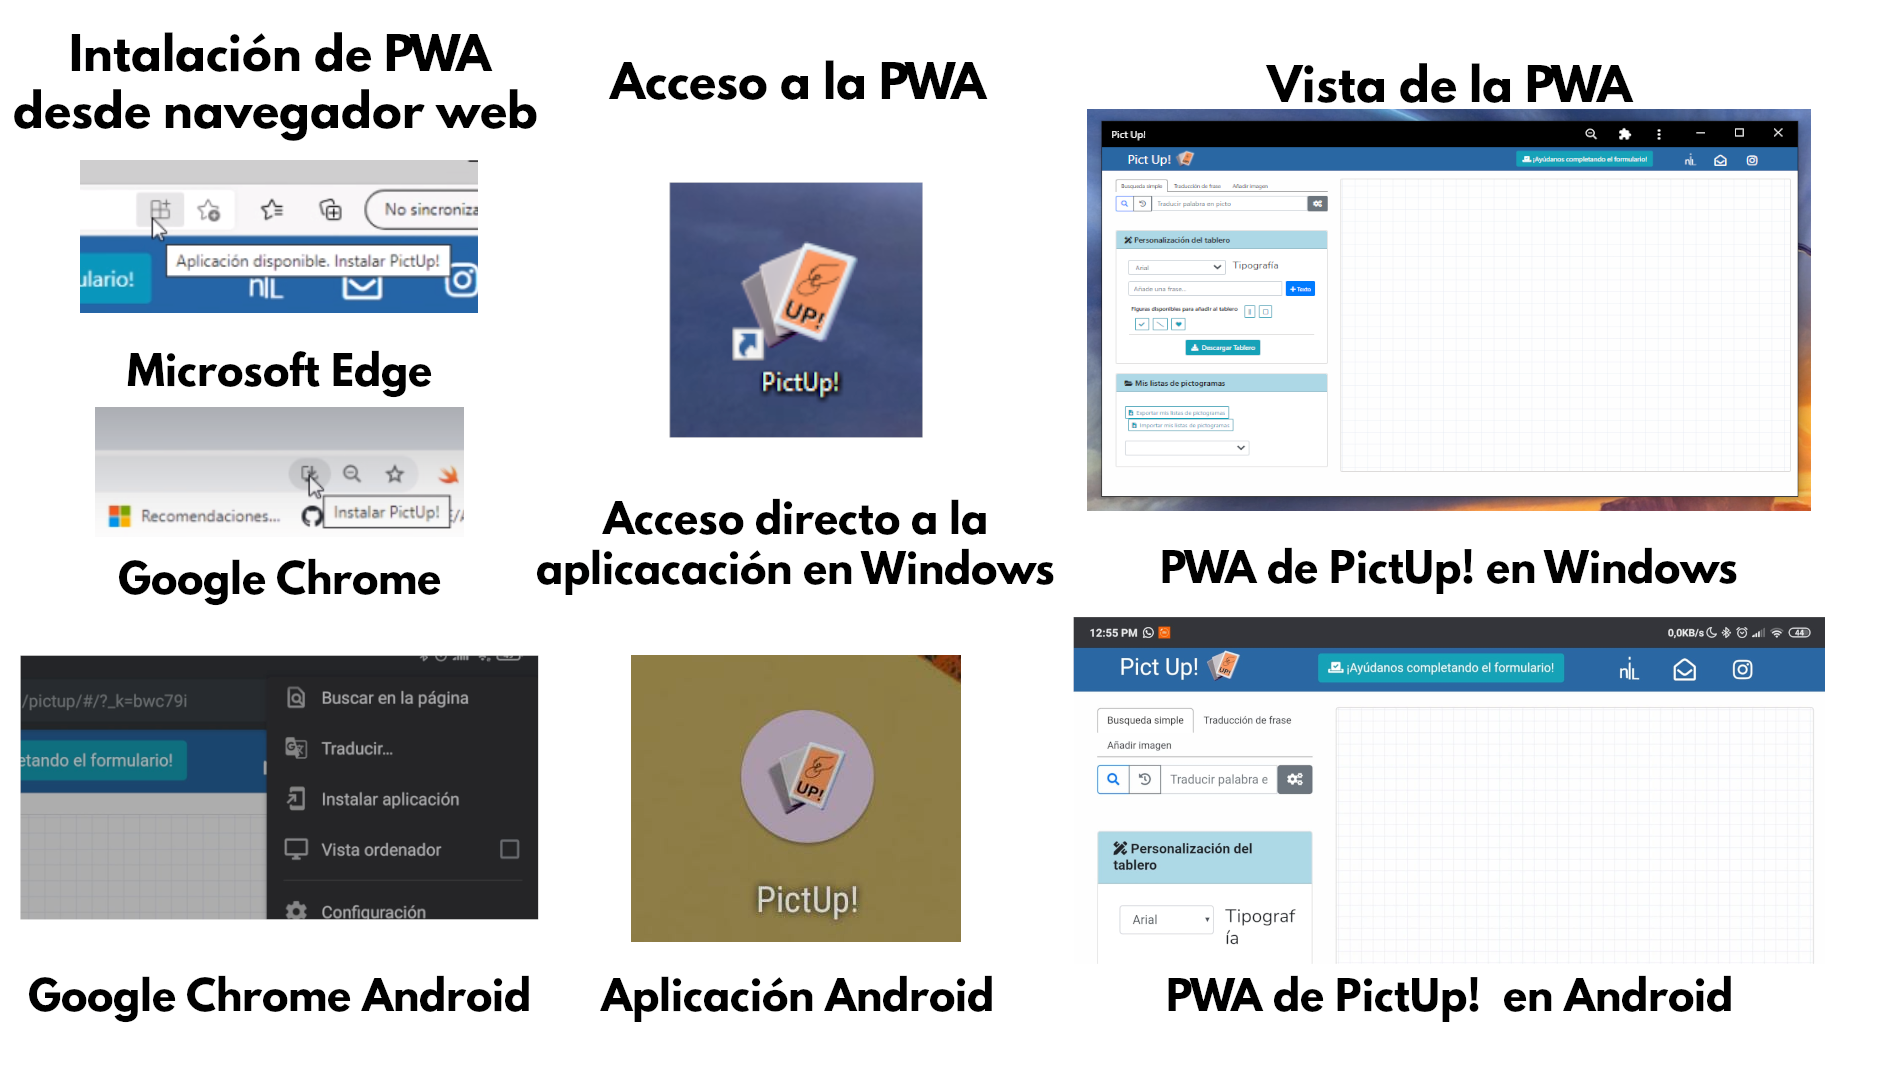
\includegraphics[width=\linewidth]{Imagenes/Bitmap/pwa}
	\caption{Esquema de instalación y uso de PWA.}
	\label{fig:pwa}
\end{figure}

Por último mencionar que el servicio de traducción de pictogramas de  NIL-WS-API, pese a encontrarse en el mismo servidor, al realizar una petición de traducción aunque no provocara un error de \textit{CORS} visto anteriormente, tampoco retornaba ninguna respuesta.

\section{Control de versiones y organización del desarrollo de PictUp!}
\label{cap5:controlversiones}

Para gestionar el desarrollo de la aplicación de PictUp!, el código de esta se encuentra en el repositorio de GitHub de NIL Group\footnote{\url{https://github.com/NILGroup/TFG-2021-EditorPictogramas}}. Gestionar de esta manera el proyecto ayudó a poder tener un mejor control de versiones y ver qué modificaciones se habían realizado en cada versión.

Para facilitar el reparto de tareas entre los dos integrantes, se utilizó un Kanban donde se especifican las funcionalidades a implementar. Cuenta con cuatro columnas, dependiendo del estado del desarrollo de cada funcionalidad: pendiente, en desarrollo, pruebas y completado. Tras acabar todas las funcionalidades principales, se creó otro Kanban donde se detallaron errores que dificultan la interacción y usabilidad de cara a una futura evaluación con usuarios. 






